%%%%%%%%%%%%%%%%%%%%%%%%%%%%%%%%%%%%%%%%%%%%%%%%%%%%%%%%%%%%%%%%%%%%%%%%%%%%
% FILE    : VTank.tex
% SUBJECT : Master document for the VTank documentation set.
% AUTHOR  : (C) Copyright 2010 by Vermont Technical College
%
%%%%%%%%%%%%%%%%%%%%%%%%%%%%%%%%%%%%%%%%%%%%%%%%%%%%%%%%%%%%%%%%%%%%%%%%%%%%

% ++++++++++++++++++++++++++++++++
% Preamble and global declarations
% ++++++++++++++++++++++++++++++++
\documentclass{report}


% --------
% Packages
% --------
\usepackage[pdftex]{graphicx}
\usepackage{listings}
\usepackage{hyperref}
\usepackage{rotating}

% The following are settings for the listings package
\lstset{language=C++,
        basicstyle=\small,
        stringstyle=\ttfamily,
        commentstyle=\ttfamily,
        xleftmargin=0.25in,
        showstringspaces=false}


% ------------------
% Layout adjustments
% ------------------
\pagestyle{headings}
\setlength{\parindent}{0em}
\setlength{\parskip}{1.75ex plus0.5ex minus0.5ex}


% ------
% Macros
% ------
%%%%%%%%%%%%%%%%%%%%%%%%%%%%%%%%%%%%%%%%%%%%%%%%%%%%%%%%%%%%%%%%%%%%%%%%%%%%
% FILE    : macros.tex
% SUBJECT : File to hold the macros defined in the VTank project.
% AUTHOR  : (C) Copyright 2009 by Vermont Technical College
%
%%%%%%%%%%%%%%%%%%%%%%%%%%%%%%%%%%%%%%%%%%%%%%%%%%%%%%%%%%%%%%%%%%%%%%%%%%%%

% ------------
% New Commands
% ------------

% Add commands in alphabetical order.
\newcommand{\command}[1]{\texttt{#1}}    % For formatting commands.
\newcommand{\filename}[1]{\texttt{#1}}   % For formatting file names.
\newcommand{\newterm}[1]{\textit{#1}}    % For formatting terms when they are first introduced.
\newcommand{\GameServer}{Theater}				 % Holds the game server's name.
\newcommand{\Janitor}{Janitor}					 % Holds the database manager's name.
\newcommand{\MainServer}{Echelon}				 % Holds the main server's name.
\newcommand{\BackupServer}{Silica}       % Holds the backup server's name.
\newcommand{\WebServer}{Porkbarrel}      % Holds the web server's name.
\newcommand{\MapEditor}{Gardener}        % Holds the map editor's name.
\newcommand{\Client}{VTank}
\newcommand{\placeholder}{\textit{placeholder\ldots}}  % To make it easy to find.
\newcommand{\VTank}{VTank}               % For formatting ``VTank.''
\newcommand{\xml}[1]{$<$#1$>$}           % For formatting an XML element inline.
\newcommand{\Launcher}{Launcher}			   % Holds the launcher's name.
\newcommand{\Patcher}{Patcher}			     % Holds the patcher's name.
\newcommand{\FormWrap}{NeoForce}         % Holds the form wrapper used for the client
\newcommand{\AI}{AI Framework}		       % Name of the AI framework.
\newcommand{\WeapProps}{Weapons.xml}             % Name of the xml file for weapon properties.
\newcommand{\ProjProps}{Projectiles.xml}         % Name of the xml file for projectile properties.
\newcommand{\EnvProps}{EnvironmentProperties.xml}         % Name of the xml file for environment properties.

% Versioning
% The following commands encapsulate the versions used for easy editing in the future.
\newcommand{\BoostVersion}{1.39}
\newcommand{\IceVersion}{3.4}
\newcommand{\MiKTeXVersion}{2.7}
\newcommand{\PCLintVersion}{9.0}
\newcommand{\StacklessPythonVersion}{2.6.1}
\newcommand{\TeXnicCenterVersion}{1 Beta 7.50}
\newcommand{\XNAVersion}{3.1}


% ----------------
% New Environments
% ----------------

% An environment to display a sequence of commands.
\newenvironment{commands}
  {\begin{quote} \tt}
  {\end{quote}}


% An environment for displaying use cases.
%   This environment takes three parameters:
%   \param #1: The name of the use case.
%   \param #2: The actor who participates in the use case.
%   \param #3: The context in which the use case executes.
%
%   The body of the environment is the action associated with the use case.
\newsavebox{\UseCaseName}    % Create some boxes to hold the necessary text.
\newsavebox{\UseCaseActor}   % We need to do this because we can't use the
\newsavebox{\UseCaseContext} % environment parameters in the 'end' definition.
\newsavebox{\UseCaseAction}
\newenvironment{usecase}[3]
 {
  \sbox{\UseCaseName}{\bfseries #1}  % The name is easy.
  \sbox{\UseCaseActor}{#2}           % The actor is easy.
  \begin{lrbox}{\UseCaseContext}     % Format the context in a minipage.
    \begin{minipage}{3.25in}
    #3
    \end{minipage}
  \end{lrbox}
  \begin{lrbox}{\UseCaseAction}      % The environment body becomes the action.
  \begin{minipage}{3.25in}}
 {\end{minipage}
  \end{lrbox}
\begin{center}   % Now spew forth the table using the information collected above.
\begin{tabular}{|l||p{3.5in}|} \hline
\multicolumn{2}{|c|}{\usebox{\UseCaseName}} \\ \hline
Actor   & \usebox{\UseCaseActor}   \\ \hline
Context & \usebox{\UseCaseContext} \\ \hline
Action  & \usebox{\UseCaseAction}  \\ \hline
\end{tabular}
\end{center}}


% ------------------
% Various TeX macros
% ------------------

% Macros that allow authors to easily insert initialed comments.

% Chris
\long\def\cbnote#1{\marginpar{CB}{\small \ \ $\langle\langle\langle$\
{#1 -- CB}\
    $\rangle\rangle\rangle$\ \ }} 
    
% Peter
\long\def\pcnote#1{\marginpar{PC}{\small \ \ $\langle\langle\langle$\
{#1 -- PC}\
    $\rangle\rangle\rangle$\ \ }} 
    
% Andy
\long\def\asnote#1{\marginpar{AS}{\small \ \ $\langle\langle\langle$\
{#1 -- AS}\
    $\rangle\rangle\rangle$\ \ }} 
    
% Michael
\long\def\msnote#1{\marginpar{MS}{\small \ \ $\langle\langle\langle$\
{#1 -- MS}\
    $\rangle\rangle\rangle$\ \ }} 
    
% Brian
\long\def\msnote#1{\marginpar{BH}{\small \ \ $\langle\langle\langle$\
{#1 -- BH}\
    $\rangle\rangle\rangle$\ \ }} 
    
% Rob
\long\def\rwnote#1{\marginpar{RW}{\small \ \ $\langle\langle\langle$\
{#1 -- RW}\
    $\rangle\rangle\rangle$\ \ }} 

% Trevor
\long\def\twnote#1{\marginpar{TW}{\small \ \ $\langle\langle\langle$\
{#1 -- TW}\
    $\rangle\rangle\rangle$\ \ }} 
    
% Isaac 
\long\def\ipnote#1{\marginpar{IP}{\small \ \ $\langle\langle\langle$\
{#1 -- IP}\
    $\rangle\rangle\rangle$\ \ }} 
    


% +++++++++++++++++++
% The document itself
% +++++++++++++++++++
\begin{document}


% ----------
% Title page
% ----------
\title{\VTank\ Documentation}
\author{Summer of Software Engineering}
\date{Summer 2010}
\maketitle


% -----------------
% Table of contents
% -----------------
\pagenumbering{roman}
\tableofcontents
\newpage
\pagenumbering{arabic}


% ----------------
% Document content
% ----------------
\chapter{Introduction}
\label{intro}
VTank is an on-line multi-player tank game. While the player need only run an installer to play VTank, administrators have several components to set up before this instance of the VTank world becomes playable. This document targets technically sophisicated users interested in setting up and configuring all parts of VTank. This document focuses on what's required to install and configure VTank servers and environments. However, this document will not address the design or architecture of the VTank world. For a detailed technical overview on the VTank world, please view the main PDF available at: \url{http://vtank.cis.vtc.edu/development/}.

\section{Obtaining the source code}
\label{src}

The source code of VTank is required in order to compile and build certain parts of the game. As of this writing, the method for obtaining the source code for VTank is to use a Subversion client to check out the following url:

\command{svn://svn.cis.vtc.edu/VTank/trunk/}

VTank may move to an alternate version control engine in the future. The latest method of obtaining the source code is available at the following URL under the ``Source Code'' section:

\url{http://vtank.cis.vtc.edu/development}

\section{Environment Variables}
\label{env-variables}

There are several times throughout the VTank install process where environment variables should be added or modified. This section shows how to do that, and instructs on which variables should be added.

\label{procedure-modify-properties}
The following procedure shows how to modify/add environment variables:
\begin{enumerate}
	\item Open up the Start menu.
	\item Right-click on ``My Computer'' (or just ``Computer'' on Windows 7 and Vista) and go to Properties.
	\item \emph{Windows 7}: On the left-hand side, left-click on ``Advanced system settings.''\\
	\emph{Windows XP}: Go to the ``Advanced'' tab.
	\item On the bottom of the System Properties, left-click on the ``Environment Variables...'' button.
\end{enumerate}

This screen shows a list of environment variables for your computer. Each variable may contain multiple entries separated by a semi-colon (\command{;}) mark. The following environment variables should be added or modified:

\begin{itemize}
	\item \command{ICEROOT} - The location of where you installed Ice. For example, if you installed Ice to \command{C:/lib/Ice}, \command{ICEROOT} should be set to \command{C:/lib/Ice}.
	\item \command{PATH} - Modify your \command{PATH} system variable. Scroll to the end of the variable's value. At the end of it, place this string:\
		\command{;\%ICEROOT\%/bin;}
	\item \command{PYTHONPATH} - If this variable already exists, modify it. If not, create it. Append to the variable the following string:\
		\command{\%ICEROOT\%/python}
\end{itemize}

\section{Visual Studio}

As of this writing, 3.1 is the most recent version of XNA. XNA 3.1 does not support Visual Studio 2010. At least Visual Studio 2008 is required in order to compile Theater, the game server. If you do not wish to compile the client, you may use Visual Studio 2010, but Visual Studio 2008 is at minimum required to compile parts of VTank necessary to run an instance of VTank.

Visual Studio is a commercial product. If you work in an educational environment you may have access to a student license. If you are a student with a \command{.edu} mailing address, you may get Visual Studio 2008 or 2010 for free at:

\url{https://www.dreamspark.com/}

Otherwise, Visual C++ Express is adequate to compile Theater, and Visual C\# express is adequate to compile Captain VTank (if you desire to do so).

\section{Ice}

Ice is object-oriented middleware which sits between all networked objects in the VTank world. Echelon, Theater, the client, the map editor, the administrative client, the website, and every other networked component of VTank uses Ice. Therefore, it's the first dependency that must be installed.

\subsection{Installation (Windows)}

ZeroC provides an installer for Ice on Windows. In addition, the installer installs a plug-in for Visual Studio which is required to build the VTank project. Ice's latest installer can be found at their website in the ``Downloads'' section located at:

\url{http://zeroc.com}

The installer's name will likely be formatted as:

\command{Ice-\#.\#.\#.msi}

Where the three numbers are version numbers. As of this writing, Ice uses version 3.4.1. It's generally safe to install a minor version (e.g. 3.4.*), but migration from 3.4 to 3.5 may produce compatibility problems.

{\bf It is currently required that Ice is installed under \command{C:/lib/Ice}}

%%%%%%%%%%%%%%%%%%%%%%%%%%%%%%%%%%%%%%%%%%%%%%%%%%%%%%%%%%%%%%%%%%%%%%%%%%%%
% FILE    : Architecture.tex
% SUBJECT : Document describing architecture issues in the entire VTank system.
% AUTHOR  : (C) Copyright 2009 by Vermont Technical College
%
%%%%%%%%%%%%%%%%%%%%%%%%%%%%%%%%%%%%%%%%%%%%%%%%%%%%%%%%%%%%%%%%%%%%%%%%%%%%

\chapter{Architecture}
\label{architecture}

\section{Overview}

The overall architecture of the \VTank\ system is shown in Figure~\ref{fig:arch-VTank}. The main server provides services for the entire \VTank\ system. There is only one main server for a particular \VTank\ community. Programs that are directly used by various user classes (administrators, editors, and players) all interact with the \VTank\ system through the main server.

\begin{figure}[htbp]
  \centering
  \scalebox{0.5}{\includegraphics*{Figures/Overall-Architecture.pdf}}
  \caption{Overall \VTank\ Architecture}
  \label{fig:arch-VTank}
\end{figure}

The main server stores all non-volatile data about the \VTank\ community in a back end database. This information includes account data, tank information, and game maps. All of the other programs in the \VTank\ system access this data through the main server. Thus the exact nature of the back end database is a private implementation detail for the main server.

One or more game servers manage the dynamics of the game world. Multiple game servers are provided for load sharing. They are managed by the main server on behalf of user commands but players also interact directly with the game servers while playing the game.

Users interact with the \VTank\ system in several ways, using different programs as appropriate. Players use the client program. Users who are creating maps (game worlds) use the map editor program. Administrators use the Captain \VTank\ program. A Janitor program also exists that allows specially designated users limited access to database administrative functions. In principal this capability could be implemented as part of Captain \VTank. However, by providing it as a separate program we can keep the user interface uncluttered and improve security.

In addition there are plans to provide a web interface (not shown above) to certain administrative actions provided by the Captain \VTank\ and Janitor programs. This web interface is likely to be minimal at first, but it has the potential to completely replace Captain \VTank\ and the Janitor. A web version of the client (for example, running in Silverlight) has also been discussed.

\section{Security}

\VTank\ is a multi-player network game. It is the nature of such a game that not all of the players may trust each other. In addition malicious users who are not players may attempt to disrupt or control a game in progress by manipulating the network over which the game is being conducted. It is therefor desirable for \VTank\ to provide some degree of security against these threats. This section outlines the issues involved in \VTank\ security. Specific information about how security related matters have been implemented is given in later chapters.

\subsection{Threat Model}

The general environment in which a \VTank\ game is taking place is assumed to be potential hostile. Specifically the analysis of \VTank's security makes the following assumptions:

\begin{enumerate}
\item Players do not trust other players.
\item Servers do not trust players (or the client programs acting on their behalf).
\item The network is hostile and in the control of a Dolev-Yao attacker. Such an attacker has the following capabilities:
  \begin{enumerate}
  \item Able to read all packets everywhere simultaneously.
  \item Able to modify any packet.
  \item Able to inject new packets on any link.
  \item Able to record arbitrary amounts of network data and replay it anywhere at any time.
  \item Able to block, delay, or rearrange packets on any link.
  \end{enumerate}
\item The attacker has full access to the \VTank\ source code (both client and server) and any predefined constant data stored by either client or server.
\end{enumerate}

In order for a reasonable security system to be designed, some trust and some limitations on the attacker's capabilities must be assumed. Specifically:

\begin{enumerate}
\item Players trust servers (once the server has been authenticated).
\item Servers trust each other (once they have mutually authenticated).
\item The Dolev-Yao attacker can not:
  \begin{enumerate}
  \item Read or modify computations done on any legitimate machine.
  \item Break any cryptographic algorithms used.
  \end{enumerate}
\end{enumerate}

Note also that the data transferred between client and server or between servers is not considered confidential (with the exception of password or other authentication information). Thus encrypting that data on the network is not necessary.

There are several threats that VTank should counter. Specifically:

\begin{enumerate}
\item A player should not be able to log in as another player. A player should only be able to modify his/her own profile or tank status, and then only to the degree allowed by the server. Note that an administrative user may exist who is exempt from this limitation; administrators can modify the profile and tank status of any player.

\item It should not be possible to disrupt a game in progress by introducing bogus packets on the network, or by replaying previously recorded packets.

\item It should not be possible for a player to use a rogue client program to cheat or otherwise gain an advantage in the game. It should not be possible for a player to use a rogue client program to disrupt a game in progress.
\end{enumerate}

Note that \VTank\ does not need to protect itself against attacks involving blocked packets. A Dolev-Yao attacker will be able to disrupt a game by causing network communication failure. However, \VTank\ clients and servers should make an attempt to detect such a situation and alert their users accordingly.


%%%%%%%%%%%%%%%%%%%%%%%%%%%%%%%%%%%%%%%%%%%%%%%%%%%%%%%%%%%%%%%%%%%%%%%%%%%%
% FILE    : ToolsLibraries.tex
% SUBJECT : Document describing the tools and libraries used by VTank.
% AUTHOR  : (C) Copyright 2016 by Vermont Technical College
%
%%%%%%%%%%%%%%%%%%%%%%%%%%%%%%%%%%%%%%%%%%%%%%%%%%%%%%%%%%%%%%%%%%%%%%%%%%%%

\chapter{Tools and Libraries}
\label{toolslibraries}

This chapter describes the tools and libraries used in the \VTank\ development environment. Both
where to get the necessary components and how to set them up are covered here. This chapter is
only of interest to \VTank\ developers. If you are a \VTank\ player or administrator you do not
need to read this chapter. Instead the details for setting up the components of a working
\VTank\ system are described in Chapter~\ref{deployment} on Deployment.

The following list reflects the tools and libraries used by the \VTank\ developers.

\begin{itemize}
\item Boost \cite{boost}
\item Dia \cite{dia}
\item DirectX SDK
\item Dynamic Model Viewer
\item Ice \cite{ice}
\item Map Previewer
\item MySQL
\item NSIS
\item NUnit
\item Stackless Python
\item Threadpool \cite{threadpool}
\item Visual Studio 2015
\item wxWidgets \cite{wxWidgets}
\item XACT
\item XNA Framework
\item xWinForms
\end{itemize}

\section{Boost}

Boost is an advanced collection of C++ libraries originally intended as a testing ground for
facilities that might one day become part of the C++ standard \cite{boost}. The libraries in
Boost are peer reviewed and are generally of high quality. They also take advantage of many
advanced C++ features to provide a degree of elegance one rarely finds in ordinary C++
libraries.

The \VTank\ project uses Boost freely in the two C++ projects, \GameServer\ and \MapEditor.
Building either of these projects requires that you install Boost. Developing either of these
projects requires that you be familiar with at least some of the Boost libraries such as
\lstinline!boost::smart_ptr! and \lstinline!boost::thread!.

The official version of Boost used by the \VTank\ project is version \BoostVersion. Other nearby
versions are likely to work; many Boost libraries do not change much between versions. Of course
for maximum compatibility with the existing \VTank\ code base we recommend that you install
precisely version \BoostVersion.

Many of the Boost libraries are expressed as templates and thus are entirely contained in their
header files. These libraries do not need to be explicitly compiled. They are effectively
compiled each time the header files are included. However some Boost libraries, notability
\lstinline!boost::thread! and \lstinline!boost::regex!, do have supporting implementation files
that need to be compiled separately.

While it may be possible to download compiled Boost binaries for Windows or Linux (for example
using your Linux distribution's package manager), we recommend building Boost from scratch.
Ultimately this gives you more control over the configuration of the library and it ensures that
the library as built corresponds properly to the other tools and libraries you are using. We
give a summary of the build instructions, with \VTank\ related notes, below. Note that we
currently only describe the build on Windows. Linux development is not officially supported, but
it should be easy to adapt these instructions for that environment as well.

\subsection{Windows}

To build Boost perform the following steps.

\begin{enumerate}

\item Download the Boost library from the Boost web site \cite{boost}. Unpack it to some
  suitable location on your system. To satisfy \VTank\ build requirements you will need to set
  the BOOST\_HOME environment variable to point at this location. We recommend that you make
  this a system environment variable and reboot your machine to ensure that it takes effect
  globally before trying to build \VTank. Note, however, that BOOST\_HOME is not required by
  Boost itself and so you can continue building Boost (below) without it.

\item Open a Visual Studio Developer Command Prompt so that access to the Visual C++ command
  line tools is available.

\item In the root of the Boost source tree (\%BOOST\_HOME\%) execute the command
\begin{commands}
bootstrap
\end{commands}

This command builds the \command{bjam} tool used to do the rest of the build. The resulting
executable \filename{bjam.exe} (or \filename{b2}) is left in \%BOOST\_HOME\%.

\item Use \command{b2} to build the various libraries. For example, just issuing:
  \begin{commands}
    .$\backslash$b2
  \end{commands}

  will build everything. This gives you maximum flexibility in that you can use whatever Boost
  libraries you need without further build steps.

\item For projects that require Boost add \$(BOOST\_HOME) to the include paths and
  \$(BOOST\_HOME)/stage/lib to the linker library paths.

\end{enumerate}

\section{wxWidgets}

\subsection{Windows}

The GUI components of \MapEditor\ are handled using the well known wxWidgets library
\cite{wxWidgets}. Version \wxWidgetsVersion\ of wxWidgets is the recommended version. Note that
the wxWidgets installer only installs the source code of the library. After running the
installer it is still necessary to compile the source using Visual C++.

Unfortunately the latest version of wxWidgets at the time of this writing (version 3.0.2) does
not support Visual Studio 2015. However, it can be made to work anyway by editing
\filename{src/tiff/libtiff/tif\_config.h} at line 367 in the wxWidgets source. Change:

\begin{verbatim}
#define snprintf _snprintf
\end{verbatim}

to the following:

\begin{verbatim}
#if (defined(_MSC_VER) && (_MSC_VER < 1900))
  #define snprintf _snprintf
#endif
\end{verbatim}

When you build wxWidgets you will also notice a number of warnings related to the unrecongized
compiler version. Presummably these issues will be fixed with the next release of wxWidgets that
will fully support the Visual Studio 2015 compiler. See the discussion here for more
information:

\vspace{1.0ex}
\centerline{\url{https://forums.wxwidgets.org/viewtopic.php?t=40491}}

The most straightforward way to build the necessary library files is to change to the
\filename{build/msw} folder in the wxWidgets distribution and issue the command\footnote{If you
  have the QNX development system also installed on your computer, but sure to erase the
  contents of the MAKEFLAGS environment variable before issuing the \command{nmake} command.}:

\begin{commands}
nmake /f makefile.vc
\end{commands}

This command will build the debug static version of wxWidgets with Unicode support. We recommend
using Unicode support because it enforces a more rigorous handling of characters and strings.
This in turn creates a higher quality application. It will also facilitate creating an
international version of \MapEditor\ in the future. Accordingly the various \MapEditor\ build
control files assume a Unicode configuration.

You should also build the release version of wxWidgets with the command

\begin{commands}
nmake /f makefile.vc BUILD=release
\end{commands}

The debug and release versions can coexist without conflict. In fact, the wxWidgets library can
be built for multiple compilers simultaneously. Thus if you intend to also use Code::Blocks on
\MapEditor, you can compile wxWidgets using the MinGW version of gcc that comes with
Code::Blocks in addition to using Visual Studio\footnote{Although not a supported configuration
  you can most likely develop \MapEditor\ using Code::Blocks on Windows. See the supplementary
  document \filename{CodeBlocks-on-Windows.txt} for more information.}.

You may install wxWidgets anywhere you like. However, the Visual Studio project file provided
with \MapEditor\ assumes that you have set an environment variable named WX\_HOME that points to
the top folder of your wxWidgets installation. Note that this environment variable is not a
required part of the wxWidgets installation; it exists only for \MapEditor\ project files.

\subsection{Linux}

\textit{This subsection needs review and may be out of date.}

\MapEditor\ development is supported on Linux using gcc. However, because of the large variation
in Linux systems, no single set of instructions is likely to be appropriate for all possible
Linux distributions. Use the instructions here as a guide. You may have to make some significant
changes to them in order to get everything working on your particular system.

Both \MapEditor\ and the Code::Blocks IDE require wxWidgets. It is not essential that they use
the same version of wxWidgets, but you may find it convenient for them to do so (especially if
you are installing both wxWidgets and Code::Blocks manually). These instructions assume such a
configuration.

You may be able to install either or both of wxWidgets and Code::Blocks using your
distribution's package manager. There are advantages to taking such an approach. However, if you
are interested in developing \VTank, we recommend that you compile both products from source.
This will give you more control over their configuration and allow you to use precisely the same
versions as the other \VTank developers. In the long run, this will simplify your development.
The following steps describe what must be done to manually set up wxWidgets on a typical Linux
system.

\begin{enumerate}

\item Download \filename{wxGTK-2.8.9.tar.gz} from the wxWidgets web site. Unpack it in a
  suitable location (for example, \filename{/usr/local/src}).

\item Follow the installation instructions in \filename{install-gtk.txt}. Basically this entails
  creating a \filename{buildgtk} subdirectory and then, inside that subdirectory configure as
  follows:

\begin{commands}
../configure -with-gtk --enable-unicode --enable-monolithic
\end{commands}

The \command{--enable-unicode} and \command{--enable-monolithic} options are both needed by
Code::Blocks and \MapEditor.

\item After configuring, do \command{make} and then \command{make install}. The installation
  will be put into \filename{/usr/local/include} and \filename{/usr/local/lib}, etc.

\item Repeat the procedure in step \#2 except using a \filename{buildgtkd} subdirectory. Add
  \command{--enable-debug} to the configure command line. This creates the debugging version of
  the library. When you issue \command{make install} the debugging library will be installed
  alongside the non-debugging library. The two libraries can coexist.

\item Run the \command{ldconfig} tool to build a new shared library cache reflecting the
  additions you just made.

\end{enumerate}

NOTE: If you do make install on the release version of wxWidgets and then the debug version, it
will be the debug version of the \command{wx-config} helper program that is actually installed.
This means that wxWidgets projects that use \command{wx-config} will end up building against the
debug version of the wxWidgets library. This may or may not be desirable. For example it turns
out that Code::Blocks v8.02 does not work with the debugging wxWidgets library. You may wish to
install the debugging version of wxWidgets first so that the final version of
\command{wx-config} is actually the release version.

Using wxWidgets in Code::Blocks projects is actually fairly simple. To access the headers use
the string \command{`wx-config --cflags`} (note back quotes) in the `Other Options' tab of the
`Compiler Settings' tab of the build options dialog. To access the libraries use the string
\command{`wx-config --libs`} (note back quotes) in the `Other Linker Options' box of the `Linker
Settings' tab of the build options dialog. You can make these changes at the top level of the
options definition. There is no need to specialize for debug and release builds. However, be
aware that this means both the debug and release versions of your program will be using
whichever version of wxWidgets is reported by \command{wx-config} (see the previous paragraph
for more on this issue).

\section{CruiseControl.NET}

Note that if you install IIS after installing the .NET Framework you will need to explicitly install ASP.NET v2 into your IIS system. The IIS installer does not do this automatically\footnote{However, the .NET Framework installer will install ASP.NET into your IIS system if IIS is already installed when the .NET Framework is installed.}. To take care of this detail manually, open a VS2008 command prompt (this assumes you have Visual Studio installed already) and issue the command

\begin{commands}
aspnet\_regiis -i
\end{commands}

The C++ components of \VTank\ use a custom unit test framework. You will need to configure CC.NET in a special way before it will understand how to execute and display the unit tests that use this framework. Specifically, in the CC.NET configuration file, inside the sections for the \GameServer\ and \MapEditor\ projects, include the following \xml{exec} task immediately after the \xml{msbuild} task.
\begin{verbatim}
<exec>
  <executable>check.exe</executable>
  <baseDirectory>Debug</baseDirectory>
  <buildArgs>check.xml</buildArgs>
</exec>
\end{verbatim}

It is important to include this task after the \xml{msbuild} task so that it executes only if the \xml{msbuild} task executes first and completes successfully.

Next in the \xml{publishers} section immediately before any XML logger tasks include the following
\begin{verbatim}
<merge>
  <files>
    <file>Debug\check.xml</file>
  </files>
</merge>
\end{verbatim}

This will combine the unit test results into CC.NET's overall build log where they can be subsequently analyzed and displayed.

Finally, in order for the results of the unit tests to be displayed properly on the web dashboard it is necessary to install an appropriate XSL file into the web dashboard's configuration. In the root of the web dashboard application, edit the file \filename{dashboard.conf}. In the \xml{buildReportBuildPlugin} element, add an \xml{xslFile} child element that names \filename{UnitTestManager.xsl}. Copy this file into the \filename{xsl} subfolder. Note that the existing reference to \filename{unittests.xsl} should not be removed. That XSL file formats the test output from NUnit or JUnit. Since this configuration change applies to all projects and since some \VTank\ projects use NUnit, it is necessary for both unit test formatting transformations to be present.

It might be desirable at some point to configure the dashboard so that each project has unique settings for the \xml{buildReportBuildPlugin} element. With the configuration described here it is necessary to ignore one of the unit test sections in each project (both are always displayed even though only one is used per project).

Note that it is necessary to restart IIS after changing \filename{dashboard.conf} in order for the changes to take effect.

\subsection{Creation of a Client}

The \VTank build script creates a new release client every time there is a successful build. Five main steps accomplish this task. 
\begin{enumerate}

\item Build Release version of the VTank
\item Kill the IcePatch2 server via PSKill
\item Update the new \Client\ files via the script UpdateClientFiles.bat
\item Build a new distribution of Patcher files via MakePatcherDistribution.bat
\item Restart the IcePatch2 server

\end{enumerate}

These are all run in order in our build script, as to make sure corrupt files don't make their way to the customer via the patcher.

\section{\LaTeX}

The primary \VTank\ documentation is written using the \LaTeX\ typesetting system \cite{latex}. This system provides high quality output with an input format that is friendly to software development tools and methods. All \VTank\ developers are expected to have some familiarity with \LaTeX\ so that they will feel comfortable editing the documentation as their work unfolds.

Although it is likely that the \VTank\ documentation could be compiled as-is on a Linux system with \LaTeX\ installed, we assume that all documentation will be edited on Windows using the MiKTeX version \MiKTeXVersion\ \cite{miktex}. Installation of MiKTeX is straight forward and essentially entails downloading the installer and running it. Here are a few notes about this process.

\begin{enumerate}

\item MiKTeX can be installed in a manner where it downloads packages on demand as they are first used. This approach minimizes the amount of disk space initially used by the system with the disadvantage of requiring Internet access when compiling a document that uses a new package for the first time. Alternatively one can do a ``complete'' installation where all packages are installed initially. This consumes a lot of disk space but it also means that any document can be compiled at any time without Internet connectivity.

\item It is convenient to include the MiKTeX bin folder on your path. This folder is
\begin{commands}
C:$\backslash$Program Files$\backslash$MiKTeX 2.7$\backslash$miktex$\backslash$bin
\end{commands}

This allows you to execute the various \LaTeX\ compilers and associated tools from the command line if desired. Some \LaTeX\ aware editors assume this ability in order to compile documents for you. Note that the MiKTeX installer may automatically take care of setting up your path for you.

\item It is probably a good idea to get in the habit of updating your MiKTeX installation periodically. From the Start Menu go to ``MiKTeX 2.7'' and then ``Update.'' The updater will identify packages that are available for updating and automatically download and install them.

\item On some machines at some times the installation or update of MiKTeX fails with a message like ``unable to write to the cache.'' This message is (most likely) from \command{fc-cache}, a tool used to create the font cache for \command{xetex}. If you are not using \command{xetex} (and \VTank\ does not) you can ignore this error. However, you can also try executing \command{fc-cache} from the command prompt manually. This often corrects the problem (the issue appears to be related to the execution of \command{fc-cache} under the control of the installation utility). For example
\begin{commands}
fc-cache -f -v
\end{commands}
The community appears to be uncertain as to why this problem occurs.

\end{enumerate}

In addition to \LaTeX\ itself you will also want to install a \LaTeX\ editing environment. In theory you can use any text editor. In fact many editors (Emacs, Notepad++, etc) have special \LaTeX\ editing modes to make the preparation of \LaTeX\ documents easier. However, the official \VTank\ environment for editing \LaTeX\ documents is TeXnicCenter version \TeXnicCenterVersion\ \cite{texniccenter}. This program provides an IDE-like environment for working on \LaTeX\ documents, complete with a project facility and many menu items for selecting various \LaTeX\ environments and features.

The installation of TeXnicCenter is straight forward. Note, however, that you should install MiKTeX first so that TeXnicCenter can auto-detect it and configure itself appropriately. If you install TeXnicCenter first, you will need to manually configure the various output profiles later.

The use of TeXnicCenter is mostly self evident. To edit the \VTank\ documentation, open the file \filename{VTank.tcp} in the \filename{Docs} folder. This is the TeXnicCenter project file for the \VTank\ documentation. From here you can navigate to the other files as needed and build the final PDF by clicking on the ``build output'' button on the top TeXnicCenter tool bar (it's near the center).

MiKTeX comes with the necessary tools out of the box to build PDF and PostScript output. To view this output you will need a PDF viewer and a PostScript viewer. Note that at this time the \VTank\ documentation only requires PDF tools. However, you may wish to install PostScript support as well for other \LaTeX\ projects.

The widely used Acrobat PDF viewer works perfectly well, but you may want to consider a different viewer that does not hold the PDF file open all the time. This allows you to keep the document on display while you compile a new version of the document. With Acrobat, the compilation will fail if Acrobat is displaying the file because Acrobat locks the file. A viewer that works better in this situation is SumatraPDF (it is also open source).

The open source Ghostscript and its associated viewer GSView work well for displaying PostScript files.

 
\section{PC-Lint}

PC-Lint is a commercial static analysis tool for C++ by Gimpel Software \cite{pc-lint}. At the time of this writing the \VTank\ developers are using the latest patch release of PC-Lint version \PCLintVersion, applying the tool to the two C++ projects in VTank: \GameServer\ and \MapEditor.

PC-Lint is very configurable and, in fact, creating the detailed configuration files needed by the tool is a considerable amount of work. Thus the precise PC-Lint configuration used with \VTank\ is checked into the repository where it can evolve along with the rest of the code base. Although the PC-Lint installer will help you set up a default configuration, this is useful only if you intend to apply PC-Lint to other projects. The configuration created by the installer is ignored when you apply PC-Lint to \VTank.

In each folder where PC-Lint can be used the file \filename{LIN.BAT} runs PC-Lint assuming that it has been installed in the default location. However, it directs PC-Lint to \VTank\ specific configuration files. The \filename{lint-config} folder off the root of the \VTank\ source tree contains general configuration information that applies to all \VTank\ projects. Note that in \filename{lint-config} the files \filename{options.lnt} and \filename{std.lnt} contain \VTank\ customizations. All other files in that folder are intended to be identical to those provided in the PC-Lint distribution.

In addition, \filename{LIN.BAT} includes a project specific configuration file that is customized for each \VTank\ project. For example the project specific configuration for \MapEditor\ is in \filename{Map\_Editor.lnt} in the \MapEditor\ root folder. In most cases, adjustments to the PC-Lint configuration should be done in this project specific file. This allows individual \VTank\ projects to use PC-Lint to enforce different polices. The project specific configuration is also the appropriate place to include annotations about project specific functions.

In addition each project contains a file containing a list of linted source files. For example the file list for \MapEditor\ is in \filename{Map\_Editor-FileList.lnt} in the \MapEditor\ root folder. This file can be given as an argument to \filename{LIN.BAT} to direct PC-Lint to process the entire program in one run. This is necessary to take advantage of PC-Lint's inter-module analysis. It is also possible to execute \filename{LIN.BAT} on one source file at a time. This would be the usual approach during development when changes to one file need to be checked.

\subsection{Usage Notes}

\VTank\ uses PC-Lint in a fairly strict mode of operation. The tool thus produces many messages when applied to ``ordinary'' C++ code. To make the burden of using PC-Lint manageable it is important to apply the tool frequently to developing code and to address the messages it produces as soon as possible. This minimizes the number of messages produced in any one run of the tool.

The ultimate goal is to evolve a PC-Lint configuration that is both strict and precise. The configuration should be strict in the sense that it should detect many common problems and force the \VTank\ developers to use good C++ programming style. The configuration should be precise in the sense that it should, to the greatest extent possible, capture complete and correct semantic information about the functions used. This will allow PC-Lint to detect real errors that would go unnoticed by an ordinary compiler.

Since building an appropriate PC-Lint configuration is itself a non-trivial undertaking, it is expected that it will take some time before that configuration is in its final state. As both the code and configuration change, the amount of output produced by PC-Lint will naturally fluctuate. Thus while it is desirable to create code that is completely ``lint free,'' it is also expected that developers will sometimes check in code that contains lint.

\emph{It is important that developers do not rush to eliminate PC-Lint output by simply disabling messages.} Often the significance of a message is not immediately obvious. What's more, when the meaning is clear it is often not immediately obvious what the best fix might be. In many cases, PC-Lint messages indicate deep design and organizational problems that go well beyond the immediate issue being diagnosed. Applying a ``quick fix'' solution, especially by disabling the message in question, will negate many of the benefits of using the tool.

\section{Ice-\IceVersion}

Ice binaries are available for download at \url{http://zeroc.com}. We recommend downloading the
offline installer and then following the platform specific instructions found here:
\url{https://zeroc.com/downloads/ice}.

\subsubsection*{Windows}

Download and execute the offline installer package for Windows. Set the environment variable
\command{ICE\_HOME} to the location where Ice was installed (information on how to do that is
not covered in this document). Some compile scripts use the \command{ICE\_HOME} variable to
locate certain binary or required slice files.

You will also want to install the Ice Builder for Visual Studio 2015. A link to the appropriate
page can be found on this page:

\vspace{1.0ex}
\centerline{\url{https://doc.zeroc.com/display/Ice36/Using+the+Windows+Binary+Distribution}}

Right-click on any project which uses Ice (e.g. the Network project), and at the bottom of the
pop-up menu you should see ``Ice Configuration...''. Selecting the ``Ice Configuration...''
option should bring up the option dialog to configure Ice for that project. Every project which
uses Ice in some way must be configured like so:

\begin{itemize}
\item Set the ``Ice Home'' field to ``\command{\$(ICE\_HOME)}'' (without the quotation marks).
\item Under the ``Ice Components'' section, check the `Ice', `Glacier2', and `IceSSL' fields at
  the bottom. This will add assembly references to these DLLs to the project.
\item Click the ``Close'' button.
\end{itemize}

These instructions are slightly different for two projects in particular: the IceCs project and
the IceCpp project. In \emph{both} of those projects, ensure the following configurations are
set:

\begin{itemize}
\item Set the ``Ice Home'' field to ``\command{\$(ICE\_HOME)}'' (without the quotation marks).
\item Under the ``Slice Include Path'', click ``Add''. Simply type a period (i.e. the current
  directory) and press Enter. Ensure that the check box which appears after you press Enter is
  unchecked.
\item Under the ``Ice Components'' section, check the 'Ice', 'Glacier2', and 'IceSSL' fields at
  the bottom. This will add references to these assembly DLLs to the project.
\end{itemize}

You will know if every project which uses Ice is not configured properly because it will
complain about missing assembly references to Ice or Glacier2. If that occurs, check the project
which reports this error, then ensure that project's Ice configuration is correct.

\subsubsection*{Ice with Python}

The following instructions were tested with Python 2.6.4. It is not guaranteed to work the same
in any other versions.

Edit the \command{PYTHONPATH} environment variable to include the following paths:

\begin{itemize}
\item \%ICE\_HOME\%\verb+\+bin
\item \%ICE\_HOME\%\verb+\+python
\end{itemize}

Note that you may need to use the x64 folder in your paths in the case of a 64 bit operating
system:

\begin{itemize}
\item \%ICE\_HOME\%\verb+\+bin\verb+\+x64
\item \%ICE\_HOME\%\verb+\+python\verb+\+x64
\end{itemize} 

Run the Python interpreter and type:

\command{import Ice;}

You may get an error about a missing DLL. If so, the easiest way to deal with this is to add
\command{\%ICE\_HOME\%/bin} to your \command{PATH} environment variable. Doing so will add the
DLLs for Ice to your PATH. The alternate way to deal with this is to copy all of the Ice DLLs
into the python/DLLs folder. It's important to remember to restart your terminal or your
computer if necessary after making modifications to environment variables.

\subsubsection*{Linux}

\emph{Note: These instructions may not work correctly with VTank. VTank administrators now
  compile Ice manually on Linux machines. This documentation will be updated in the future.}

Linux machines with \filename{yum} installed can view Ice packages from the Ice repository.
ZeroC provides a more detailed explanation regarding exactly how to install and update Ice
automatically and from RPM packages at:

\vspace{1.0ex}
\centerline{\url{http://www.zeroc.com/download.html\#linux\_rpms}}

The \filename{yum} installer will install all of the Ice binaries and files required to run
Python under the default installation of Python. You may have to compile Ice yourself if you are
not using the default installation of Python.

\section{Threadpool}

Threadpool is a third-party addon to the Boost library that leverages the
\lstinline!boost::thread! class to create functionality similar to Stackless Python. Each
`thread' in the threadpool is actually a customized task. Rather than creating a separate thread
for each task inside of the pool, the tasks are executed in a concurrent fashion. The tasks are
not run in parallel to each other. \pcnote{This doesn't sound right. The documentation says the
  tasks do execute in parallel.} Instead, it uses a scheduler to decide which tasks it should
execute and when. Therefore, if a certain set of data is only accessed by one threadpool, it
does not require thread safety. \pcnote{A conclusion that might be false. Check this!} Every new
threadpool created uses a \lstinline!boost::thread! to run the scheduler.

\subsubsection*{Windows}

Installing the Threadpool library is relatively easy. The project is available on sourceforge at
the address: \url{http://threadpool.sourceforge.net}. On the front page, scroll down to the
section labelled as `Download Section'. Download the source (the package ending in `src.zip') by
clicking on the link.

Threadpool can be extracted anywhere you prefer. In Visual Studio, add the Threadpool include
directory and the boost directory that was extracted with Threadpool. Since Threadpool uses the
Boost.Thread library, the \filename{libboost\_thread-*.lib} library is required to be linked. It
is preferable to add a \%THREADPOOL\_HOME\% environment variable so that everyone is not
required to install the source in the same location on their PC.

\section{MSTest Testing} 

\subsection{Description}
MSTest is a software unit testing framework developed by Microsoft, which integrates closely with Visual Studio. We are currently using this framework for adding unit testing to the VTank Client. The executable is included with any Visual Studio installation. 

The testing framework is contained in a separate project within the Client solution called ClientTests. The test project file structure mirrors the Driver structure, so each class file that needs tests has a corresponding test file in the same folder. So a file in Client/src/utils/Class.cs has a test file in ClientTests/test/utils/ClassTest.cs.

\subsection{Overview of adding a test}

When you add a new class to the Client Project, you must create a new class in the ClientTests project. The naming convention for the new class is the original classname followed by the word "Test". So a class called Foo would have a corresponding test class called FooTest. The new class must include using statements corresponding to the original file namespace and also to "Microsoft.VisualStudio.TestTools.UnitTesting"; 

MSTest uses a series of attributes so that the compiler will know that the class/methods are testing classes/methods. So right above the class name, place the attribute [TestClass]. Some tutorials have it shown as [TestClass()], however it doesn't matter to the compiler, so we use the attribute without the (). 

Now you have a solid base to begin coding your unit tests. 

To create unit tests for a particular method, create a method in the test class with the same name followed by the word "Test". So a method in Foo called Bar that needs testing, should have a corresponding method in FooTest called BarTest. This is the naming scheme used by SoSE for testing individual methods, but it doesn't matter to the compiler. If you wish to group several methods in the same test for instance, you may name it something more meaningful. 

The test method must also have a corresponding attribute above it called [TestMethod]. 

The way MSTest checks the output of methods is through "Assert" statements. Assert contains several definitions of different tests, such as Assert.IsTrue or Assert.IsNull. You can use these statements to perform your unit testing. The following method is a sample of what you can do while testing an addition function. 
\lstset{frame=shadowbox}
\begin{lstlisting}
[TestMethod]
public void AddTest()
{
     int result = Add(5, 6);
	
     Assert.AreEqual(result, 11);
     Assert.AreNotEqual(result, 32);
}  
\end{lstlisting}

For more complicated tests, MSTest has built in support for creating a reusable harness for all your tests. If you are going to be using an object multiple times over a variety of tests for instance, you can specify a initialization method that can either initialize it before all tests or before every test. For example, if you wanted to initialize a couple integers before testing several math methods, you could place it in a [ClassInitialize] method. 

\begin{lstlisting}
int x;
int y;
       
[ClassInitialize]
public static void MyClassInitialize(TestContext tc)
{
     x = 7;
     y = 2;
}
\end{lstlisting}

If you are going to modify said integers within the test method, you would want them to be reset to their original values prior to each test, so you would add a [TestInitialize] method that gets executed before every test method is run. 

\begin{lstlisting}
[TestInitialize]
public static void MyTestInitialize()
{
     x = 7;
     y = 2;
}
\end{lstlisting}

Both the ClassInitialize and TestInitialize attributes have cleanup methods associated with them: ClassCleanup and TestCleanup respectively. The TestCleanup method is called after each test that is run, and the ClassCleanup method is called after all tests are completed. Below is a full example test file for a Math class with an Add method. 

\begin{lstlisting}
/*!
    \file   MathTest.cs
    \brief  Example MSTest file
    \author (C)Copyright 2009 by Vermont Technical College
*/

using System;
using Microsoft.VisualStudio.TestTools.UnitTesting;
using Client.src.utils.Math;

namespace ClientTests.src.utils
{
[TestClass]
public static class MathTest
{
int x;
int y;
		
[ClassInitialize()]
public static void MathTestClassInitialize(TestContext tc)
{
x = 7;
y = 3;
}

[ClassCleanup()]
public static void MathTestClassCleanup()
{
x = null;
y = null;
GC.Collect();
}
 
[TestInitialize()]
public void MathTestsInitialize()
{
x = 7;
}
 
[TestCleanup()]
public void MathTestsCleanup()
{
x = null;
}
		
[TestMethod]
public void AddTest()
{
Assert.AreEqual(x, 7);
x = Add(y, 2);
Assert.AreEqual(x, 5);
Assert.AreNotEqual(x, 32);
}  
}
}
\end{lstlisting}

\subsection{Running tests}
\subsubsection{From within Visual Studio}
\begin{enumerate}
\item Start Visual Studio and open the Client solution.
\item Right-click on the ClientTests Project in the Solution Explorer pane
\item Highlight the \textit{Debug} option in the pop-up menu, and click on the \textit{Start new instance} option when it appears. 
\end{enumerate} 
Visual Studio will take all the tests from the project and run them, displaying a nice output screen with the results. 

\subsubsection{From the Visual Studio Command Line}
\begin{enumerate}
\item Start Visual Studio and open the Client solution.
\item Build the solution. A file called \textbf{ClientTests.dll} will be built and put in the directory \textit{Client/ClientTests/bin/Debug/}.
\item Open the \textbf{Visual Studio 2008 Command Prompt} from the start menu. The default location is under \textit{Microsoft Visual Studio 2008/Visual Studio Tools/Visual Studio Command Prompt}
\item Navigate to the \textbf{Debug} directory as described above. 
\item Run the command \textbf{MSTest} with the following flags \textit{/testcontainer:ClientTests.dll /resultsfile:testResults.trx} . This will run all of the tests in the project and display them in a nice text-based format. 
\end{enumerate} 

\section{XACT}

\subsection{Description}

Microsoft's cross-platform audio creation tool (XACT) is a highlevel audio library for creating and playing audio using DirectSound. XACT Auditioning Utility is a companion tool that organizings the sound and wave files into banks to be later played back using the XACT project solution in an XNA project. The XACT project solution should be referenced in the Content folder.

NOTE:
This utility has to be running while XACT is opened to get the program to work correctly. The tool can be found in the XNA SDK under tools. If it is not running when XACT is, just simply start it and then in XACT click on the 'Audition' tab and 'Connect to Local' this will connect to the auditing tool and the editing and auditing of music will work as intended.

\subsection{XACT Project}

\subsubsection{Creating an XACT project}

Open up the XACT program in the XNA SDK folder and click on the File - New Project. Call this file anything relative to what the audio is in reference to.

\subsubsection{Adding Audio and Sound}

To add audio or sound to the project two banks have to be made: a wave bank and an sound bank. Once the project has been established, right click on the `Wave Bank' on the right side of the screen and select `New Wave Bank'. Do the same thing for the sound bank. Once that has been established it is time to add sound. 

XACT only supports the following audio types:
\begin{enumerate}
\item WAV
\item AIFF
\item XMA
\end{enumerate}

First begin by either right clicking in the wave bank window and select `Insert Wave File' or drag the wave file into the window.

The wave file will turn red which indicates that the sound was added but is not linked to an effect. once all the wave files have been added to the project, they must be linked ton an effect. 

Select all the wave files and drag them into the sound effect window under the `Cue Name` sub-window. This will place the same names from the wave bank in the cue and in the sound bank.

The names that appear in the cue is what XNA will refer to when it needs to call on a sound effect for play back.

If everything is done correctly the wave files in the wave bank will turn green and it is ready to compile. Select File - Build or press the `F7' key to compile the audio.

If an error stating that an audition server could not be found, start up XACT Auditioning Utility program and try again.

\subsubsection{XACT Runtime Parameter Controls (RPC)}

XACT's Runtime Parameter Controls or RPC defines how 3D audio will be heard to the client. In the XACT project there are global variables that are defined and can be modified.

\begin{enumerate}
\item SpeedOfSound
\item Distance
\item DopplerPitchScalar
\item NumCueInstances
\item OrientationAngle
\end{enumerate}

All these variables can be modified to produce desired effects. The most important one is the Distance. This sets the distance between the Audio Emitter and Audio Listener.

Right click on RPC Presets and select Apply new RPC. It will bring up a new window. Select the variable that you want to control in the drop down menu (Distance for example). Under `Option' drop down window select sound and `Parameters' Volume. Next a graph will show a vertical line. This line represents what the sound will do when the distance changes. Double click on the line will add a new point and can be modified to change what happens at that distance. Preferably the first point should be placed in the upper left corner of the map and the last point in th lower right. This will make it that if the listener is on top of the emitter the client will hear the full sound. Once the client has moved away the sound will diminish as the distance changes. Messing with the points between the begin and end  points will change what happens as the distance changes. Adjust these points until the desired effect is obtained.  

\subsubsection{Removing Audio and Sound}

To remove the audio and sound effects from an XACT project, simply click on the wave file to remove and press the delete key. This will have to be done in both the sound bank and wave bank to remove reference to the audio from the project then re-compile the project.

\subsubsection{Adding XACT to an XNA project}

To add an XACT project to XNA, simply drag the XACT project solution into the Content folder in the XNA project solution. It is recommended to create an audio folder in the Content directory to reference the audio.

\subsubsection{Loading XACT Sound in XNA}

Three variables will be needed to reference sound in an XNA project:

\begin{enumerate}
\item \texttt{AudioEngine}
\item \texttt{SoundBank}
\item \texttt{WaveBank}
\end{enumerate}

The \texttt{AudioEngine} is the driving force for the sound. This is the device that references the XACT file.

An example to implement the audio engine is as follows:

\texttt{AudioEngine audioEngine = new AudioEngine(``Content/audio/VTankAudio.xgs'');}

\texttt{Content/audio/VTankAudio.xgs} points to the directory where the XACT project is located and the reference to the sound bank and wave bank files.

After the audio engine has ben established it is time to initalize the \texttt{SoundBank} and the \texttt{WaveBank}.

\texttt{SoundBank soundBank = new SoundBank(audioEngine, ``Content/audio/soundbank.xsb'');}
\texttt{WaveBank waveBank = new WaveBank(audioEngine, ``Content/audio/wavebank.xwb'');}

Both the soundBank and the waveBank variables take the audioEngine as a parameter which points to the XACT project that holds information on the sound bank and wave bank files.

\subsubsection{Playback}

All play backs of audio or sound effects is done in the soundBank. To play a sound back simply type \texttt{soundBank.PlayCue(sound);}

\texttt{sound} is a string that targets to the Cue name specified in sound banks cue section of the XACT project.

When an event that is  previously specified happens and the play back is called then the soundBank will reference the cue with the given string name to find the file to play back to the user.

\subsubsection{Adding 3D Audio}

XNA supports 3D audio. This support allows clients to hear sound depending on their position and where the sound comes from. This is established by creating an audio emitter and an audio listener. The audio emitter is given the position and the velocity of the projectile while the listener is set to the clients position. Each sound is then prompted to apply the 3D audio effect and passed in the listener.

For example:

\texttt{AudioListener listener = new AudioListener();}

\texttt{AudioEmitter emitter = new AudioEmitter();}

This sets defines the listener and the emitter. \texttt{listener.Position} is set to the position of the client and \texttt{emitter.Position} is set to the projectile being fired. This establishes the distance between the listener and emitter to determine how the audio will be heard to the client.

After that is established a Cue is created for the selected sound effect to be played.

The \texttt{soundBank} is called to get the desired cue to be played

\texttt{Cue cue = soundbank.GetCue(``Explosion'');}

Next we can call the \texttt{Apply3D} to pass the cue the listener and the emitter.

\texttt{cue.Apply3D(listener, emitter);} 

Once that is established then the audio will be updated and the sound will change according to the position of the client.


\section{NSIS}

\subsection{Description}
NSIS (Nullsoft Scriptable Install System)\cite{nsis} is the tool used by VTank to generate the Windows installer. This section will include a basic description of how to make a NSIS script and what it takes to build your own VTank installer. 

\subsection{NSIS Scripting}
Visit \href{http://nsis.sourceforge.net/}{NSIS homepage} and download the latest version of NSIS and install it on your system. 

\subsection{Make your own VTank installer}

In the trunk of the VTank project there is a script called PatcherInstall.nsi, which is the main script for creating a VTank distribution. This script depends on several files to be present in order to compile properly. This section will walk you through the steps necessary to compile this script. 

\begin{enumerate}
\item \texttt{If you haven't yet, download and install NSIS (see above section).}
\item \texttt{Check out the VTank project from the Subversion server}
\item \texttt{Build the VTank project in Release mode in Visual Studio.}
\item \texttt{Run the Make\_Patcher\_Distribution.bat file in the /Client/Patcher/ directory. This will copy all the necessary executables and support files needed to run VTank.}
\item \texttt{Copy the file xnafx31\_redist.msi (available \href{http://www.microsoft.com/downloads/info.aspx?na=90&p=&SrcDisplayLang=en&SrcCategoryId=&SrcFamilyId=53867a2a-e249-4560-8011-98eb3e799ef2&u=http\%3a\%2f\%2fdownload.microsoft.com\%2fdownload\%2f5\%2f9\%2f1\%2f5912526C-B950-4662-99B6-119A83E60E5C\%2fxnafx31_redist.msi}{here}) to the root directory of the project folder (The same place where PatcherInstall.nsi is located) This file is the XNA redistributable that gets bundled with our installer.}
\item \texttt{Right click on the PatcherInstall.nsi script and select "Compile NSIS Script". This will launch the NSIS compiler and produce a VTankPatcherSetup.exe in the same directory as the install script.}
\end{enumerate}

Note: An alternative way to compile: 
\begin{enumerate}
\item \texttt{Open the NSIS program from the start menu.}
\item \texttt{Click on the option on the top left named "Compile NSI scripts" under the Compiler header.}
\item \texttt{This will open a program called MakeNSISW. You can use this program to browse the file system and open the script you want to compile, or just drag and drop the script onto this window.}
\end{enumerate}


\section{XNA}

"Microsoft XNA is a set of tools with a managed runtime environment provided by Microsoft that facilitates computer game development and management." VTank uses version \XNAVersion\ . In order to run games created with XNA, you will need at minimum the basic XNA redistributable. In order to build VTank from scratch however, you will need the full SDK distribution in the form of an extention to Visual Studio. Both are available at Microsoft's website. 

Note: If you install VTank from our installer, the XNA redistributable is bundled and will install automatically when you run it. 

\section{DirectX SDK}
The DirectX SDK is another set of tools that Microsoft provides for the development of any applications that use DirectX as their graphics driver.  XNA being directX based, you will also need the DirectX SDK installed in order to compile VTank.  VTank uses the \DirectXSDKVersion\ version of DirectX.  The DirectX SDK is available in the \href{http://msdn.microsoft.com/directx/}{DirectX section of Microsoft's MSDN website}.

In addition to being a dependency for VTank, the DirectX SDK also provides tools for model/texture viewing, among other things.  Note, however, that at this time VTank only supports .fbx files, which cannot be viewed in the DirectX viewer.
 
\section{Blender}

Blender is currently the 3D modelling tool of the project. It is a powerful open source, cross platform tool. This section contains the protocols  on creating, texturing, animating and exporting 3D models for use with VTank. 

\subsection{Installing and Configuring Blender for XNA}
\begin {enumerate}
\item {Download Blender.}
To get blender, go to the  \href{http://www.blender.org/download/get-blender}{Blender Download Page}. Make sure to download the zip archive (currently Blender 2.49b Zip Archive) instead of the executable. Once this is downloaded, extract it and Blender is good to go.
 
\item {Check your Computer for Blender's requirements.}
Blender 2.49b requires Python 2.6. Make sure that you have it.

\item {Install the Custom .fbx Exporter.}
For VTank models, the official file format is .fbx. Blender's packaged .fbx exporter doesn't mesh well with XNA. The link to a custom .fbx for XNA exporter can be found in the \href{http://wiki.blender.org/index.php/Extensions:2.4/Py/Scripts/Export/FBX-xna}
{Blender Wiki}
or, for a direct link, go to
\url{http://www.triplebgames.com/export_fbx__for_xna.py}.

\begin{enumerate}
	\item Copy and Paste this text into a text editor
	\item Save the file in Blender-Root-Folder / .blender / scripts
	\item Make sure the Autodesk FBX(.fbx) Modified for XNA exporter is available in Blender
\end{enumerate}

\end {enumerate}
\subsection {Creating and Exporting Models for VTank}
\subsubsection {Orientation and Scale}

\begin{table}[h]
	\centering
		\begin{tabular} {l | r}
		 Up & Positive Z \\
		 Front & Positive Y\\
			
		\end{tabular}
\end{table}

Currently, the axis that faces the camera in VTank is the positive-Z axis, and the axis that faces angle 0 (or the front of the tank or turret) is the positive-Y axis. If you insert a basic cube mesh and scale it 15 times you get the general height of a tank model. 
\begin{figure}[h]
	\centering
		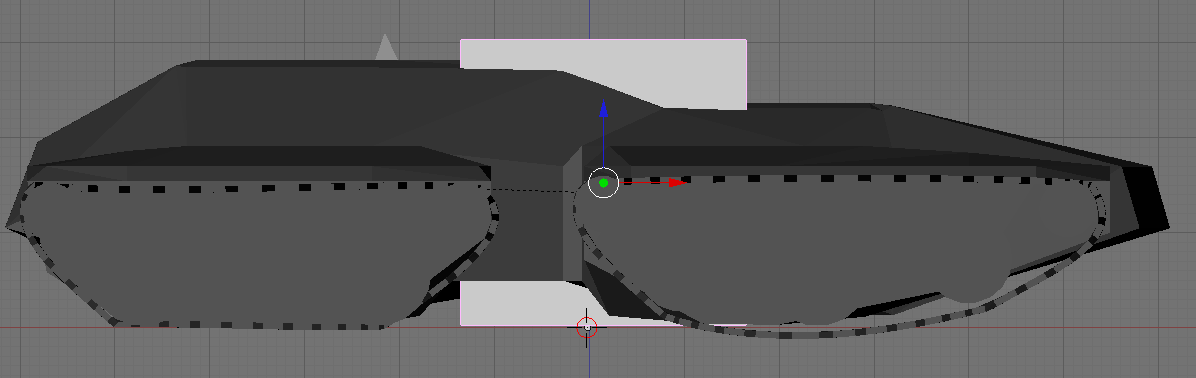
\includegraphics[width=0.50\textwidth]{Figures/tankAndCube.png}
	\caption{A tank and  x15 scale cube}
	\label{fig:Scale Sample}
\end{figure}


\subsubsection {Modelling Tips and Tricks}
Very good blender tutorials can be found in the \href{http://en.wikibooks.org/wiki/Blender_3D:_Noob_to_Pro}{Blender Noob to Pro Tutorials}.

\subsubsection {Naming Conventions}
\textit{Mesh Conventions}

Mount : This is the position where an object that is attached to the current mesh will be placed. See the pyramid where the turrent will be attacehd to the tank in Fig 3.1.

Color : Any mesh named Color will change color depending on the player's settings.

Cannon0 : The gun barrels should be named Cannon0. For multiple cannons start with Cannon1, Cannon2 etc.

Emitter0 : This is the position where projectiles will be generated from a mesh. For multiple emmitters user Emitter1, Emitter2 etc. 

\textit{Model Conventions}

The name that you give a model will be the name of the unit in game (eg. Behemoth.fbx is the model for the Behemoth tank) so choose your names accordingly. Also, every tank or weapon should have an associated \_dead model that will display when the entity is destroyed in game. These should be named MODELNAME\_dead.fbx (eg. Behemoth\_dead.fbx).

\textit{Texture Conventions}

Be as specific as possible with your texture names. Follow the example modelname\_meshname\_texturename.png, where 'modelname' is the name of the associated .fbx file (ex. Cannon), 'meshname' is the name of the specific mesh this texture will be applied to (ex. GunBarrel0), and 'texturename' is a description of the type of texture (ex. Forestgreen\_Rusted).


\subsubsection {Texturing}
XNA only supports UV texturing. UV involves making seams in your mesh so that blender can cut along then and unwrap your 3d mesh onto a 2d surface. You then draw an image or upload and image onto this surface. Blender will map the image to your model with respect to the faces in the unwrapped mesh. This sounds complicated but is actually very easy.

\begin{enumerate}
	\item Apply a different material to every part of model that requires a different texture.
	\item Right click on top of viewing panel and select 'Split Area'.
	\item Select 'UV / Image editor' from the box in the lower left corner of the new window.
	\item In the original window, select the part of your model you want to texture on and enter Edit Mode.
	\item Select the edges that you want Blender to use as seams, press 'CTRL + E' amd select 'Mark Seam'.
	\item Select entire area, press 'U' and select 'Unwrap'. The 'UV / Image editor' window should now display a flattened version of your model.
	\item Edit the flattened image until you are ready to draw on it. Keep in mind that highly visible areas on your model should not have seams and similar sized polygons in 3D should be represented by similar sized polygons in 2D.
	\item Export the 2D wireframe by following 'UVs / scripts / Save UV Face Layout'.
	\item Create a texture using the wireframe as a reference in an image editor. Note: Image size must be a power of 2 (ie. 256, 512 and 1024).
	\item Import your image in the UV editor by following 'Image / Open'.
\end{enumerate}

You are done. Preview your texture by changing the viewpoint shading to Textured in the 3D object window. 

Note: If you move the verticies or change the model after importing an image you will probably need to re-export the 2D wireframe and remake the texture.

Follow these steps for each other area you want to texture.

\subsubsection {Exporting for VTank}
Your model must follow a specific set of rules in order to display correctly in VTank. Be aware that 'Main' mesh refers to the main body of your model and not a mesh named Main.

\begin {enumerate}
\item {\bf Your model conforms to the Orientation, Scale, Naming, and Texturing protocols. }
\item {\bf Your model has no change in Scale or Rotation from it's ObDATA. }\\
\begin{itemize}
	\item Enter 'Object mode'
	\item Select all objects by pressing 'A'
	\item Pess 'CTRL + A' and select 'Scale and Rotation to ObData'
\end{itemize}

Note: If you rotate or scale your model again, you must repeat this step. 

\item {\bf The main mesh's center is placed correctly.Y}\\
Placing the center is very important, as it is the point that your model will rotate around while moving in game. It also defines where the model will rest on the ground. Keep this in mind when placing your centers. 

Method 1: 
\begin{enumerate}
	\item Go to 'Object Mode'.
	\item Select your main mesh and enter 'Edit Mode'.
	\item In 'Editing Panel' (F9) go to 'Mesh / Center New'.
	\item Select 'Object / Snap / Cursor to Selection'.
	\item Go to 'Object Mode'.
	\item Without moving the cursor, select 'Add / Mesh / Empty Mesh'.
	\item Reposition the empty mesh so it is level with the bottom of the model.
	\item Select the main mesh press 'Shift' and select the empty mesh.
	\item Press 'CTRL + J' and then 'Enter'.
	\item Rename the main mesh to it's original name.
\end{enumerate}

Note: Keep in mind that this method puts the center at the location of the empty mesh. This might not be exactly where you want your model to rotate. Use your best judgment. 

Method 2: The previous way makes it easier to place your center in the right place if your mesh is relatively balanced. Another way to place your center is to get your cursor where you want your center to be and then select your main mesh, enter 'Edit Mode', open the 'Editing Panel'(F9) and go to 'Mesh Panel / Center Cursor'. This will place the objects new center wherever you placed your cursor. You can use the 'Object / Snap' functions to make this a lot easier.

Note: Remember to re save your ObData!

\item {\bf The center for your 'Main' mesh is at the origin.}\\
Now that your model has a correct center, move your entire model so the center is at the origin of Blender's grid. Again, this is easily done with the 'Object / Snap' functions. 

\item {\bf All meshes in your model are somehow connected.}\\
Usually using the add parent function. To add a parent, first make sure that all of the meshes are in the right place and the ObData is saved, then go to object mode. Select the object that you want to make the child, then hold ShiftKey and select the object to make the parent. Now press CntrlKey+PKey and click Add Parent. 

Note: If you change anything after setting the parent you must UnParent before resaving the ObData. Do this by selecting all objects, pressing AltKey+PKey and selecting Clear Parent (Save Track).

Note: Remember to resave your ObData!

\item {\bf Export}\\
When ready, go to  File / Export / Autodesk FBX (.fbx) Modified for XNA. A box will appear. Select 'Scene Objects' and deselect 'X90'. Click export. Choose the name for your file and its destination folder and click 'Export FBX'. Make sure the export 
\begin{figure}[h]
	\centering
		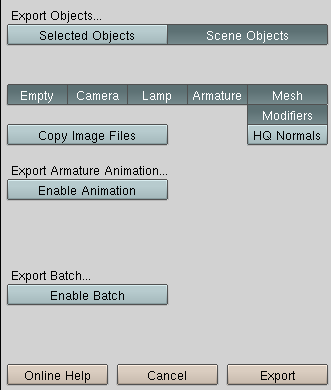
\includegraphics[width=0.50\textwidth]{Figures/ExportFBX.png}
	\label{fig:ExportFBX}
\end{figure}


\item {\bf Double Check .fbx File}\\
Sometimes, the links to your textures in the .fbx file are not correct. To fix this open the .fbx file in a text editor and search for the texture names with CtrlKEY+FKEY. Make sure that the path to the texture is correct and the texture and .fbx files are in the right place. 

\end{enumerate}

\section{Dynamic Model Viewer}

The dynamic model viewer is a tool created by the VTank team that is used by artists who want to see what their creations will look like in game without writing any code. Available in the VTank.sln file, just build it and run it. 


\begin{table}[h]
	\centering
		\begin{tabular} {l | r}
		C & Toggle camera views \\
		S & Toggle shadows \\
		L & Toggle lighting \\
		Num+ & Change percentage of day complete \\
		E & Deploy previously loaded particle emitter \\
		Ctrl + T & Load a tank model \\
		Ctrl + W & Load a weapon model \\
		Ctrl + P & Load a power up model \\
		Ctrl + E & Load a particle emitter \\
		Ctrl + A & Load an animated model \\
		Ctrl + O & Load any other model \\
		Left or Right & Rotate a Tank model \\
			
		\end{tabular}
\end{table}

The differences between loading model types only deals with how they are positioned. For instance, loading a tank and a turret will automatically attach the turret to the tank and loading a powerup will draw the model above the ground. Tanks and turrets will also vary the mesh color to show how they might look in game. 

To load a particle emitter you must load two files. The first is a particle system settings file (*.vtpss) and the second is a particle emitter settings file (*.vtpes). Also note that the texture image that the emitter uses must be a part of the project.  

\section{Map Previewer}

The map previewer is another tool created by the VTank team that enables users to preview what a map looks like ingame.  It was created to make up for the fact that our map editor only represents 2d tiles an icons, which do not adequately convey a map's actual appearance.  The map previewer puts you behind a cactus model, and allows you to 'drive' around a given map, inspecting what it looks like, without having to upload it to the active map rotation.

The controls are similar to VTank controls, with a few differences.

\begin{table}[h]
	\centering
		\begin{tabular} {l | r}
		F & Load a Map \\
		W & Forward \\
		A & Rotate Left \\
		S & Backward \\
		D & Rotate Right \\
		Spacebar & Toggle Chase / Overhead \\
		Up Arrow & Tilt Up \\
		Left Arrow & Tilt Left \\
		Right Arrow & Tilt Right \\
		Down Arrow & Tilt Down \\			
		\end{tabular}
\end{table}

Note that a map can be loaded again without closing the map previewer, enabling you to continue working on your map in \MapEditor, and reload the map when you want to see your changes.

Unfortunately, the map previewer is not associated with the main VTank project, but it can be downloaded freely from the \href{http://vtank.cis.vtc.edu/downloads}{VTank Website}, just below the download for \MapEditor.
%%%%%%%%%%%%%%%%%%%%%%%%%%%%%%%%%%%%%%%%%%%%%%%%%%%%%%%%%%%%%%%%%%%%%%%%%%%%
% FILE    : MainServer.tex
% SUBJECT : Document describing design issues in the VTank Server.
% AUTHOR  : (C) Copyright 2009 by Vermont Technical College
%
%%%%%%%%%%%%%%%%%%%%%%%%%%%%%%%%%%%%%%%%%%%%%%%%%%%%%%%%%%%%%%%%%%%%%%%%%%%%

\chapter{\MainServer}
\label{mainserver}

\section{Requirements}

\MainServer\ is a central connection point for any type of \VTank\ client. This includes not only the game client, but clients connecting from websites, from management programs such as the \Janitor, and from administrative programs such as Captain \VTank. \MainServer\ will also act as a proxy between the client and the database, which is to say that only \MainServer\ will have direct access to the database. This section describes the main server's responsibility.

\subsection{Functional Requirements}

\MainServer\ acts as an initial meeting place between a regular game client and a game server. Once \MainServer\ is started, it will receive connections from game servers, which will request a spot on the main server's list of game servers. This list is presented to each client as they connect, giving them the option to choose which game server they wish to play on.

Once a client chooses to join a certain game server, the main server will generate a SHA-1 hash from a random number salted with the client's account name and last login date. The hash is then passed to the game server and to the client. This acts as the client's key to start playing on the game server. Even after a client has started playing a game, the main server must continuously monitor it's behavior. The client is responsible for pushing ``keep alive'' messages to the main server in order to prevent it from being kicked due to inactivity.

In addition to game clients, \MainServer\ is responsible for allowing privileged members log in to perform special actions. The following types of clients are allowed to log in:
\begin{enumerate}
\item Users of developer privilege or higher are allowed to view, add, modify or delete in-game equipment (i.e. weapons, armor, projectiles) via \Janitor.
\item Administrative users will log in through Captain \VTank. Administrators are granted the following abilities:
	\begin{enumerate}
	\item View a complete list of clients.
	\item Kick any client for any reason.
	\item Ban any client for any reason.
	\item View, add, modify or delete accounts. (Administrators may not view passwords.)
	\item Disable or enable a game server.
	\item View in-depth statistics or health reports generated by \MainServer.
	\item Any action that \Janitor\ can do.
	\end{enumerate}
\item Public users through non-specific clients may request certain non-privileged information from \MainServer\ (i.e. a list of in-game clients, the current \VTank\ game client version, etc.).
\end{enumerate}

\subsubsection*{Statistics Tracking}

\MainServer\ tracks certain information for each user. There are two categories of information that \MainServer\ tracks:
\begin{enumerate}
	\item Usage-related information, such as login frequency, last login time, creation date, etc..
	\item Game-related information, such as kills, deaths, wins, losses, and ``experience points''.
\end{enumerate}
Usage-related information is for high-level accounting purposes and has no affect on the game. In contrast, game-related information affects the game in a significant way. It is \GameServer's job to calculate how many points are earned for each accomplishment. However, only statistics sent from an ``approved'' \GameServer\ instance are recorded in \MainServer's database.

Each user has a column of statistics called 'points'. Points are used as a measurement unit to determine what rank the user is placed at. Each user's tank is given an individual rank, which is raised by performing well in games to gain points. After certain thresholds as determined by the server, the tank will be promoted to a new rank. Promotion holds the following effect on users:
\begin{enumerate}
	\item New items or tank chassis may be opened up for use.
	\item Certain bonuses may apply during games.
\end{enumerate}
In addition to individual tank ranks, special ranks are also tied to a user's account to measure overall performance (that is, statistics across multiple tanks). Promotions are harder to attain for accounts and their effect on the game is currently undetermined.

Points and promotion thresholds are currently arbitrarily calculated. Approved servers are allowed to set the point values of each type of accomplishment. For instance, \GameServer\ may decide that kills are worth 20 points, flag captures are worth 100 points, and assists are worth 10 points. However, the final calculated point gain for each player is only a ``recommendation'' to \MainServer: \MainServer\ may decide to ignore those values. When \GameServer\ submits it's calculated values, \MainServer\ checks the values for validity and records them into the database. Because \GameServer\ also sends player statistics such as kills and assists, \MainServer\ may decide to completely ignore the point values received by \GameServer\ and calculate things it's own way, and indeed, if \GameServer\ is calculating too little or too many points, \MainServer\ will ignore \GameServer's recommended point calculation.

\subsection{Non-Functional Requirements}

\subsubsection*{Platform}

\MainServer\ is written in Stackless Python and does not depend on certain operating system functions. \MainServer\ will run on any platform that meets the following requirements:
\begin{enumerate}
\item Supports Stackless Python \StacklessPythonVersion.
\item Supports Ice \IceVersion\ (Python \StacklessPythonVersion\ support required).
\item Supports mysql-python, a Python package which supports MySQL communication.
\end{enumerate}

\subsubsection*{Performance}

Because slow performance in the main server does not affect \VTank's gameplay, \MainServer\ does not have strict performance requirements. However, it is preferable that it has less-than-a-second response time. The performance may be slowed considerably if the backend database's performance is abysmal or if it takes too long to communicate with the main server (which can happen if the database is not on the same machine).

The main server requires very little memory and CPU time.

\subsubsection*{Security}

The main server acts as the initial connection point for every client, including game servers, and most actions require authentication from each of these clients, including administrative clients. Therefore, security in \MainServer\ is a high priority.

Every client must use IceSSL (Ice implementation of the secure socket layer) to authenticate with \MainServer. Once authenticated, actions from the client are generally considered to be non-sensitive, so SSL is not necessary once a session has been established. It should, however, be an option for some clients, especially Captain \VTank.

Passwords will be stored as a hash in a MySQL database column. Once \MainServer\ receives the password from the client via IceSSL, it performs a SHA-1 hash on it. Since the hash is considered irreversible, it would be impossible to log in using that hash if one were somehow able to steal it. The database should be on an isolated network with no access allowed except for the main server, so packet sniffing efforts are not likely to produce results.

If a user attempts to log in with one account too many times, the account will be locked temporarily (the exact time will be decided by the main server) and a notification will be sent to administrators. Subsequent attempts on that account or attempts to log in to several different accounts will result in a temporary ban of the client's IP address and administrators will be notified again. The administrator may decide to lock down an account in question pending further investigation.

Users who forget their password may request a new one from the main server. When an account is created, the user supplies an e-mail address for exactly this purpose. A new password is generated and stored in the database (after being hashed), while the password is sent to the user's registered e-mail address. If the user entered an invalid e-mail address, he is forced to contact \VTank\ support.

\subsubsection*{User Characteristics}

\MainServer\ will be run and managed by administrators, who are expected to be competent in the operating system used. The user must be familiar with passing command-line arguments into programs, editing configuration files, and must have some experience securing their system (particularly the firewall configuration).

\subsubsection*{Scale}

The main server's non-strict performance requirements mean that the main server will likely not have to expand into grid computing or server clusters.\footnote{This may change considerably if VTank gains thousands of active users.}

\subsubsection*{Data Formats}

The main server reads a custom configuration file that is formatted like most \filename{*.ini} files: with square-bracketed section names and configuration properties formatted under each section. Configuration properties are formatted like:

\begin{commands}
key = value
\end{commands}

\subsubsection*{Internationalization}

\MainServer\ configuration files, databases, log outputs and debug outputs are all in US English. There are no plans to change this currently.

\section{Design \& Architecture}

Despite the fact that \MainServer\ can handle several different types of clients, \MainServer\ handles all clients inside of one client manager. This is done for two main reasons:
\begin{enumerate}
	\item It's easier to maintain N number of types of clients under one manager.
	\item It's easier to add multiple types of clients.
\end{enumerate}

\newpage
\begin{figure}
	\centering
	\scalebox{0.50}{\includegraphics*{Figures/echelon_architecture.png}}
	\caption{Object architecture of \MainServer.}
	\label{fig:echelon_architecture}
\end{figure}

\section{Compiling}

\MainServer\ is written in Python, which is an interpreted language. Python files (\filename{*.py}) are compiled to \filename{*.pyc} files, but are still interpreted nonetheless. Python is a dynamic language, so the only way to test if the program will successfully run is to provide 100\% coverage via unit testing.\footnote{Please see the section on Testing.}

Eclipse's PyDev plugin is used to develop the Python code. Projects can be imported to Eclipse and executed from there. The program's startup file, ``\MainServer.py'', can be executed either from Eclipse or from the command line. Assuming the Python interpreter is on the PATH, the main server can be executed using the following command from the directory where ``\MainServer.py'' is located:

\begin{commands}
python \MainServer.py -s\footnote{The '-s' parameter is recommended: this dynamically compiles required Slice code.}
\end{commands}

\subsection{Ice}

Ice binaries are available for download at \url{http://zeroc.com}.

\subsubsection*{Windows}

Download the latest installer package for Visual Studio 2008. Install the package and make a note of where it's installed. Set the environment variable ICEROOT to the location where Ice was installed (information on how to do that is not covered in this document). Some compile scripts use the ICEROOT variable to locate certain binary or required slice files.

Be sure to add the \filename{\%ICEROOT\%/python/} directory to the PYTHONPATH variable. These files are needed by Python to use Ice modules. Test the Ice implementation of Python by opening the Python interpreter and running these commands:

\begin{lstlisting}
import Ice
Ice.initialize()
\end{lstlisting}

An exception will be thrown from one of these statements if Ice is not working correctly.

\subsection{Stackless Python}

Stackless is a third-party implementation of Python. It installs by itself and works exactly the same way as the regular Python installation, but adds a module named ``stackless''. A more detailed explanation on Stackless and a download is available at it's website: \url{http://stackless.com}.

\subsection{mysql-python}

mysql-python is a third-party module which assists in executing SQL statements on a MySQL database. It's available for download at: \url{https://sourceforge.net/projects/mysql-python}.

\subsubsection*{Windows}

It's very simple to install mysql-python on Windows. Simply download the latest package and execute the installer. The installer will find the latest compatible version of Python and install itself there. To test if it works, open the Python interpreter and type:

\begin{lstlisting}
import MySQLdb;
\end{lstlisting}

If an ImportError does not occur, then the package installed successfully.

\subsubsection*{Linux}

Use the following simple procedure to install mysql-python on a Linux machine:

\begin{enumerate}
\item Download the latest source of MySQL-python from \url{http://sourceforge.net/projects/mysql-python}. The source is stored as a \filename{.tar.gz} file.
\item Do ``tar xfz MySQL-python-1.2.3.tar.gz'' (being sure to use the correct version number)
\item Do ``cd MySQL-python-1.2.3'' (being sure to use the correct version number)
\item Edit site.cfg if necessary.
\item Execute: ``sudo python setup.py build''
\item Execute: ``sudo python setup.py install''
\end{enumerate}

To test if it works, open the Python interpreter and type:

\begin{lstlisting}
import MySQLdb;
\end{lstlisting}

If an ImportError does not occur, then the package installed successfully.
%%%%%%%%%%%%%%%%%%%%%%%%%%%%%%%%%%%%%%%%%%%%%%%%%%%%%%%%%%%%%%%%%%%%%%%%%%%%
% FILE    : GameServer.tex
% SUBJECT : Document describing design issues in the VTank game server.
% AUTHOR  : (C) Copyright 2009 by Vermont Technical College
%
%%%%%%%%%%%%%%%%%%%%%%%%%%%%%%%%%%%%%%%%%%%%%%%%%%%%%%%%%%%%%%%%%%%%%%%%%%%%

\chapter{\GameServer}
\label{gameserver}

\section{Requirements}

\GameServer\ is where clients using the official \VTank\ game client actually play the game. \GameServer, the game server, starts by connecting to \MainServer, the main server, by sharing a secret that only official game servers can know. That secret is determined in both server's configuration file. If the secret is correct, the game server is allowed to join \MainServer's list of active game servers.

\subsection{Functional Requirements}

Once authenticated with the main server, the game server maintains an open connection to it in order to exchange messages. \MainServer\ will communicate ``player joined'' and ``player left'' messages. In other words, it's entirely up to \MainServer\ what players are allowed to join and who should not be playing.

When a player wishes to join a game, \MainServer\ first checks if it's appropriate to do that: it must check if the game server is overloaded or if the game server is disabled (by an administrator). If allowed, both the client and \GameServer\ are given a hashed, randomly generated key. The client is responsible for sending this key to the game server in order to identity itself. If the client's key matches with the key given by the main server, the client is allowed to join the game.

\GameServer\ is responsible for managing the actual game. When a player moves around, fires a projectile, joins the game, leaves the game, enters a chat message, or dies, the game server must accept this information and run calculations determining:
\begin{itemize}
\item What action was performed,
\item if the action was legal, and
\item the result of the action.
\end{itemize}
The game server must then communicate it's conclusion to every other client.

\GameServer\ must check if players are cheating. If a client suddenly moves across the map in one movement packet, something is wrong. It's important to keep in mind that a client suddenly teleporting to a location where it seems impossible for him to be is most likely the result of the client's connection temporarily lagging. The best way to deal with these events is to assume the worst: reset the position of the client back to one that makes sense. It's not unusual for online games to do this. If the client continues to misbehave, make sure to log the behavior and kick the client off. An administrator should be able to review the log and take action against the user if necessary.

\subsection{Non-Functional Requirements}

\subsubsection*{Platform}

\GameServer\ is written in C++ with the target platform being Windows Server 2003 and Windows Server 2008. There are plans to make \GameServer\ run on Linux in the future.

\subsubsection*{Performance}

\GameServer\ has high performance needs. High latency due to poor processing speed results in an unplayable game. If the average response time to each client is over 100 milliseconds, the player will find it very noticable and will make it much more difficult to play the game.

\subsubsection*{Security}

In-game actions are not secured because the actions have nothing to do with personal information. Adding a layer of security on the socket will only increase latency.

There may be a case where a player intercepts and modifies packets sent from another player. While this has been discussed, no solution has been proposed for dealing with this.

\subsubsection*{User Characteristics}

\GameServer\ will be run and managed by administrators, who are expected to be competent in the operating system used. The user must be familiar with passing command-line arguments into programs, editing configuration files, and must have some experience securing their system (particularly the firewall configuration).

\subsubsection*{Scale}

\MainServer\ is allowed to accept an array of \GameServer\ instances. That means advanced technologies like grid computing are not necessary initially: if one server gets overloaded with users, another machine in a different location can host a game. If \VTank\ gets to the point where this is not solving issues, this strategy is expected to change.

\subsubsection*{Data Formats}

\GameServer\ uses Ice to parse properties from a configuration file. Values in the Ice configuration file are set up like:

\# Comment about the pair.
key=value

\subsubsection*{Internationalization}

\GameServer\ configuration files, log outputs and debug outputs are all written in US English. There are no plans to change this currently.

\section{Design \& Architecture}

Ice is heavily involved in the design and architecture of \GameServer\ because Ice handles all input and output for client sessions. Additionally, Ice is used to communicate with \MainServer. Figure~\ref{fig:theatre_architecture} points out that MTG\_Service - Main-to-Game Service, the class through which communication to \MainServer\ takes place - is separated from the ServerService class, which handles communication to clients. 

These are kept in separate communicators because clients in the same Ice communicator have potential to interfere with each other. For example, if \GameServer\ gets overloaded with clients and runs out of threads, it could stop responding to \MainServer, which causes a timeout and essentially ends the game. Because the communicators are kept separate however, thread starvation in the client pool will not affect the communication with \MainServer.

It has been discussed that \GameServer\ may accept Ice datagram packets in the future, which use UDP. Since the client must not have to open a firewall port in order to play the game, \GameServer\ should not distribute messages via UDP. Since most traffic travels out of \GameServer, and not to \GameServer, it's been argued that there's little benefit to doing this.

\newpage
\begin{figure}
	\centering
	\scalebox{0.50}{\includegraphics*{Figures/theatre_architecture.png}}
	\caption{Object architecture of \GameServer.}
	\label{fig:theatre_architecture}
\end{figure}

\section{Compiling}

\GameServer\ is written in C++ and relies on Ice, Boost, and Threadpool. For information on these libraries (and installing them), visit the Tools and Libraries section.

\subsection{Windows}

Double-click on the \filename{VTank.sln} file available under: \filename{svn://svn.cis.vtc.edu/VTank/trunk/}. First configure which build you desire: Debug or Release. Then, right-click on the \GameServer\ project and click on the \filename{Build...} option. This will build \GameServer\ and all of it's dependencies.  



\subsection{Linux}

\GameServer\ is compiled with an Sconstruct script. Sconstruct is a python based make system that is similar to a makefile.  This script can be found in the same folder as the game server at:

\filename{VTank/trunk/Server/Game/Driver/sconstruct}

To use this script, you must have Scons and the dependency libraries installed on your machine. After installing the dependencies and scons, you will have to edit the Sconstruct file to reflect the location of your dependencies.

There are seven constants at the top of the Sconstruct file, which should be tailored to your system's dependency locations before you attempt to compile.  

These seven are:

\begin{enumerate}
\item TARGET -- The output target for your compiled files.
\item GAMESERVER -- The location of the Driver folder for the game server.
\item ICE -- The location of your Ice include folder.
\item VTANK\_COMMON -- The location of the vtank/Common/Cpp folder on your machine, note that this means you have to have a checkout of vtank, or just this folder from \filename{svn://svn.cis.vtc.edu/VTank/trunk/Common/Cpp} to use these source to compile \GameServer\\.
\item VTANK\_ICE -- The location of the vtank/Ice folder on your machine.  Just like vtank/Common, you must have these files as well to compile \GameServer\\.  They are located at \filename{svn://svn.cis.vtc.edu/VTank/trunk/Ice/}.
\item BOOST -- The location of your boost header files.
\item THREADPOOL -- The location of your threadpool header files.
\end{enumerate}

Further down in the file, find the environment settings line, which should start like this:
\begin{verbatim}env = Environment(..)\end{verbatim}

There are a couple settings lists inside this function that must be tailored to your system:

\begin{enumerate}
\item CPPPATH -- This is a list containing the directories of your include and header files, this should many of your variables you set at the top, including ICE, VTANK\_ICE, VTANK\_COMMON, BOOST, GAMESERVER, THREADPOOL, in addition to your system's default include directory for C++.
\item LIBPATH -- This is a list containing the location of the required library files.  You must put your system's default C++ library directory here, as well as your Ice-x.x.x/lib/ folder and your Ice-x.x.x/cpp/lib folder.  These are located off of your Ice installation root.
\end{enumerate}

Now go down to the Program compilation line, which looks something like this:
\begin{verbatim}env.Program(...)\end{verbatim}

Make sure that LIBPATH in this function is the same as the one in Environment, then review the LIBS list and confirm that all of the required library files are listed there.  At the time of this writing they are:

\begin{enumerate}
\item libIce.so
\item libIceUtil.so
\item libGlacier2.so 
\item libboost \_thread-mt.so
\item libIce.so.33
\end{enumerate}

Once you are confident of your settings, issue the following command from the directory the Sconstruct script is in:

\command{scons}

Once invoked, Scons will automatically find your sconstruct script in the directory, read it, and proceed to buid \GameServer\ if your script is configured correctly.  If everything was properly configured, your build will complete successfully.  Once completed, refer to the Linux Running \GameServer\ section (below) for instructions on how to configure and run \GameServer\ in Linux.
 
\section{Running}

\subsection{Windows}

While \GameServer\ has a lot of requirements for compilation, it's very simple to execute an instance of \GameServer\ on Windows. \GameServer\ will have two executables: one for executing \GameServer\ normally (in a console window), and one for executing \GameServer\ as a service. It's up to the administrator of the Windows Server 200X machine to decide whether or not to run \GameServer\ as a service.

Starting, restarting, or stopping \GameServer\ is very simple in either case. Windows services can be viewed under the Start->Administration->Services menu. Right-clicking on the \GameServer\ field allows the administrator to start, restart, or stop the instance.

\subsection{Linux}

\textbf{Configure \GameServer}


Once you have finished compiling \GameServer\ navigate to the Server/Game/Driver directory open up the file named Config.Theatre with your preferred text editor.

Find the line that looks like this:
\begin{verbatim}GameSessionFactoryProxy=GameSessionFactory:tcp -h theater.cis.vtc.edu -p 31335\end{verbatim}
Change it to reflect the hostname (or IP of your machine).

Now find the ServerName line, which should be just below it:
\begin{verbatim}ServerName=Theater\end{verbatim}
Change it to a name of your choosing.  This is the game name that will show up in the game listing in the game and on the website.

Now go down to the Glacier2Host line, which looks like this:
\begin{verbatim}Glacier2Host=theater.cis.vtc.edu\end{verbatim}
Change it to reflect your hostname or IP.

\textbf{Set up Glacier2}

The next thing you must do is compile the slice files for your Glacier2 router. Before doing so, you must have an environment variable called ICEROOT to tell the script the location of your Ice installation.

From the terminal, issue the following command:
\command{ICEROOT=/opt/Ice-3.3.1; export ICEROOT}
**Note that your Ice installation may be located elsewhere.

Once your ICEROOT variable is set, run the \filename{compile-slice.sh} script, which is located in the \filename{VTank/Ice} directory.

After your slice files have compiled successfully, go to the \filename{Vtank/Glacier2} folder and start your glacier2 router with the \filename{start-theatre-router} script.

\textbf{Start the Server:}

Once \GameServer\ is configured and your glacier2 router is running, issue the following command from the output directory.

\command{nohup ./Theater. \&}
**The name of your executable may vary.

The nohup command tells \GameServer\ to run in the background, effectively allowing it to run as a daemon.

If everything went smoothly, you should have a process with the same name as your executable running, and your game should be visible on the game list and the website.

\section{Security}

\subsection{Overview}

At Vermont Tech, \GameServer\ is currently running on a Windows server, also bearing the name \GameServer. \GameServer\ was hardened using the guidelines defined in the SoSE Windows Server 2003 security documentation.  The following list contains the categories addressed by the hardening procedure:

\begin{enumerate}
\item Security Configuration Wizard Policy
\item Password Policy Settings
\item Audit Policy Settings
\item Windows Firewall Settings
\item User Account Settings
\end{enumerate}

\subsection{Security Configuration Wizard Policy}

The initial security settings on \GameServer\ are based on the security policy \GameServer\.xml, which was created using the Security Configuration Wizard.  The policy was applied using the principle of least privilige, then built upon by adding more detailed settings using the configuration tools for each of the corresponding categories.

\subsection{Password Policy Settings}

\GameServer\ now enforces password complexity, locks a user account out for 15 minutes after 20 invalid login attempts.  No password aging or password history settings are enabled.

\subsection{Audit Policy Settings}
\GameServer\ now collects audit logs based on the following settings:
\begin{itemize}
\item Account logon events -- Success
\item Account management -- Success
\item Directory service access -- Success, Failure
\item Logon events -- Success
\item Object access -- Success
\item Policy change -- Success
\item Privilege use -- Not auditing
\item Process tracking -- Failure
\item System events -- Success, Failure
\end{itemize}

\subsection{Windows Firewall Settings}
Windows Firewall is enabled with the following exceptions:
\begin{itemize}
\item Port 123 UDP (Time Protocol Port)
\item Port 4063 TCP  (VTank Communication Port)
\item Port 4064 TCP  (VTank Communication Port)
\item Port 42424 TCP (ASP.NET port)
\item Port 3389 (Remote Desktop)
\item "Echo request" is enabled. (Ping)
\end{itemize}

\subsection{User Account Settings}
In order to reduce the risk of a compromised Administrator account, the Default administrator account on \GameServer\ is disabled.  Day to day administration tasks are carried out by a seconday adminstrator account.  A tertiary administrator account was also created, for usage in the event that the normal admin account is compromised, or locked out.  While the complete disabling of the Administrator account creates the possibility of an account lockout DOS account on other admin accounts, the Administrator account can be re-enabled by rebooting the server in safe mode.

The default Guest account is also disabled.

%%%%%%%%%%%%%%%%%%%%%%%%%%%%%%%%%%%%%%%%%%%%%%%%%%%%%%%%%%%%%%%%%%%%%%%%%%%%
% FILE    : Client.tex
% SUBJECT : Document describing design issues in the VTank Client.
% AUTHOR  : (C) Copyright 2009 by Vermont Technical College
%
%%%%%%%%%%%%%%%%%%%%%%%%%%%%%%%%%%%%%%%%%%%%%%%%%%%%%%%%%%%%%%%%%%%%%%%%%%%%

\chapter{\Client\ (client)}
\label{client}

\section{Requirements}

\Client\ is the name of the software that the user runs to play the \VTank\ game. The software uses Microsoft XNA Framework for .NET to render 3D models and textures to the screen, and Ice to communicate with \MainServer\ and \GameServer. From a regular user's perspective, the client is able to perform two functions:
\begin{itemize}
\item Manage the user's list of tanks.
\item Allow the user to play \VTank.
\end{itemize}

\subsection{Functional Requirements}

Once the client authenticates with the main server, it is allowed to perform some session-only actions. These actions include obtaining the user's personal list of tanks, requesting to join a game server, downloading a map, and other miscellaneous actions.

\Client\ uses Glacier2. This relieves users from having to open a port to play \VTank. 

\subsection{Use Cases}

The following case allows the user to authenticate with the main server.

\begin{usecase}
  {LOGIN}
  {Any User}
  {The client has just been opened and the user has not logged in yet.}
\begin{enumerate}
\item User enters account information into the 'Username' field.
\item User enters password into the 'Password' field.
\item A dialog box will appear informing the user that it is attempting to connect with the server. The user may press a 'Cancel' button to terminate the connection attempt.
\item If successful, the state of the client is changed to the tank selection screen.
\end{enumerate}
\end{usecase}

The following case allows a user to add a new tank to their list of tanks.

\begin{usecase}
  {ADDTANK}
  {Authenticated User}
  {The client has just logged in and is viewing his list of tanks.}
\begin{enumerate}
\item User has clicked the 'Add Tank' button.
\item User filled out forms about his new tank.
\item Data is sent through to the server, which will perform the updates. On error, a dialog box is presented.
\item If successful, the user is returned to the tank selection screen with the new tank present.
\end{enumerate}
\end{usecase}

The following case allows a user to modify an existing tank.

\begin{usecase}
  {EDITTANK}
  {Authenticated User}
  {The client has just logged in and is viewing his list of tanks.}
\begin{enumerate}
\item User has clicked the 'Edit Tank' button after highlighting a tank.
\item User edited fields regarding his tank.
\item Data is sent through to the server, which will perform the updates. On error, a dialog box is presented.
\item If successful, the user is returned to the tank selection screen with the modified tank present.
\end{enumerate}
\end{usecase}

The following case allows a user to delete an existing case.

\begin{usecase}
  {DELETETANK}
  {Authenticated User}
  {The client has just logged in and is viewing his list of tanks.}
\begin{enumerate}
\item User has clicked the 'Delete Tank' button after highlighting a tank.
\item Confirm dialog is presented to user: 'Cancel' returns, 'Confirm' proceeds.
\item Data is sent through to the server, which will perform the updates. On error, a dialog box is presented.
\item If successful, the user is returned to the tank selection screen with the tank removed.
\end{enumerate}
\end{usecase}

The following case allows a user to select which \GameServer\ to play on.

\begin{usecase}
	{SELECTSERVER}
	{Authenticated User}
	{The user selected his or her tank and is ready to play}
\begin{enumerate}
\item User has clicked the 'Game Server' button.
\item List of available servers are presented to the user.
\item The user highlights which server to join and then clicks the 'Join' button to proceed.
\item If successful, the state is changed to GamePlayState.
\end{enumerate}
\end{usecase}

The following case pulls up an in-game menu.

\begin{usecase}
	{INGAMEMENU}
	{Authenticated User}
	{The user is currently playing \Client.}
\begin{enumerate}
\item User hit the 'Escape' key during game play.
\item A Menu appears with the following options
	\begin{enumerate}
	\item \textbf{Resume} - Resume current game.
	\item \textbf{Options} - Brings up the Option menu that allows users to modify in-game options except video.
	\item \textbf{Log out} - Allows the user to log out and return to the Title screen.
	\item \textbf{Exit} - Exits \Client.
	\end{enumerate}
\item The user selects one of the option.
\end{enumerate}
\end{usecase}

\subsection{Install Script}

The install script will need to package up all of the necessary files required to run the VTank Client and make an executable installer that the user can run on their home machine. It will check for previous versions of DirectX and XNA and if they are not found or are outdated, it will install the required version. 

The installer will install the VTank Client in the Program Files folder by default, although the user may specify a different location if they wish. A shortcut should be placed on the desktop and in a start menu folder. The script should also create an uninstaller that will completely remove the VTank client from the user's PC (leaving DirectX and XNA intact) and place it in VTank's start menu folder. 

\subsection{Non-Functional Requirements}

\subsubsection*{Platform}

\Client\ alone can technically run on any XNA supported platform, which means the PC, XBox 360, and Zune. The client will only run on the PC currently. There are no plans to port \Client\ to the XBox 360 or the Zune, though it has been discussed. The issue with doing so is that Ice is not available for the .NET compact framework, which XBox 360 and Zune uses. If Ice were compiled for that platform, porting \Client\ to XBox 360 and Zune would be considered much more seriously.

\subsubsection*{Performance}

\Client's performance needs are a significant issue in programming, since poor code can result in horrible frame rate. \Client\ should be able to run on modern computers, and on modern operating systems at around 60 FPS without any issues.

\Client\ is rendered in 3D and this being the case, some modern computers may have difficulty running the client. It's important to detail minimum requirements as soon as possible. The minimum requirements should allow the user to run the software with reasonable frame rate no less than 30 FPS. 

The ability to tailor video option, such as the resolution, texture quality and anti-aliasing, on a user's machine can improve frame rate and performance.

\subsubsection*{Security}

The client must use IceSSL when first connecting to the server. Once it successfully authenticates with \MainServer, the client will start using the session and will no longer require SSL.

\Client\ has very little to do in terms of security. It should definitely do error checking to prevent it from bothering the server with obviously wrong information, yet clients cannot be trusted to give correct information. The server will always assume that the client is trying to sneak something bad in. It's the client's responsibility to be honest and to adhere to server demands (such as a demand to reset the tank's position to a ``legal'' one) -- otherwise the client will be kicked.

\subsubsection*{User Characteristics}

Users of \Client\ need to have no programming or development experience whatsoever. The client will be packaged in a way that makes it simple for users to download, install, update, reinstall, or uninstall \Client. Nothing more than minimum typing experience and some experience in gaming is required.

\subsubsection*{Scale}

The client more than any other software in the \VTank\ project will use a lot of memory. It must load in the map, a weapons database, an armor database, a projectile database, 3D models, textures, skins, audio clips, and much more. The most expensive objects will be the graphics, the audio, and (most significantly) the map. The user who creates maps should be careful not to upload maps that are too large.

\subsubsection*{Texture Naming Convention}

Each model has a texture mapped to it. To recognize what texture goes to which model, a naming convention is implemented. The naming convention follows the following format:  \texttt{[TextureModelName]\_texture.png}.

\subsubsection*{Data Formats}

When a new installer for a client is produced, a new ``local'' database is generated. The database is a XML file which is stored on the client-side. It works as a look-up table for what models should be used for certain types of objects. A XML-Linq library should be created to parse that file.

\subsubsection*{Internationalization}

\Client, more than any other software, has the opportunity for internationalization. If designed carefully from the beginning, error messages, dialog box text, labels, and everything else can be abstracted into a look-up table. The table has a section called ``English'', where all messages displayed in-game are stored. The user can be allowed to switch languages if needed.

\Client\ is currently only available in US English.

\section{Design and Architecture}

\Client\ makes use of several wrappers and libraries developed in house. The progression of the Client from startup to gameplay uses an approach much like a state machine. Each state performs a different task and then transitions to the next state. Each of these states is outlined in Figure~\ref{fig:clientUML}. 

\begin{figure}
	\centering
	\scalebox{0.5}{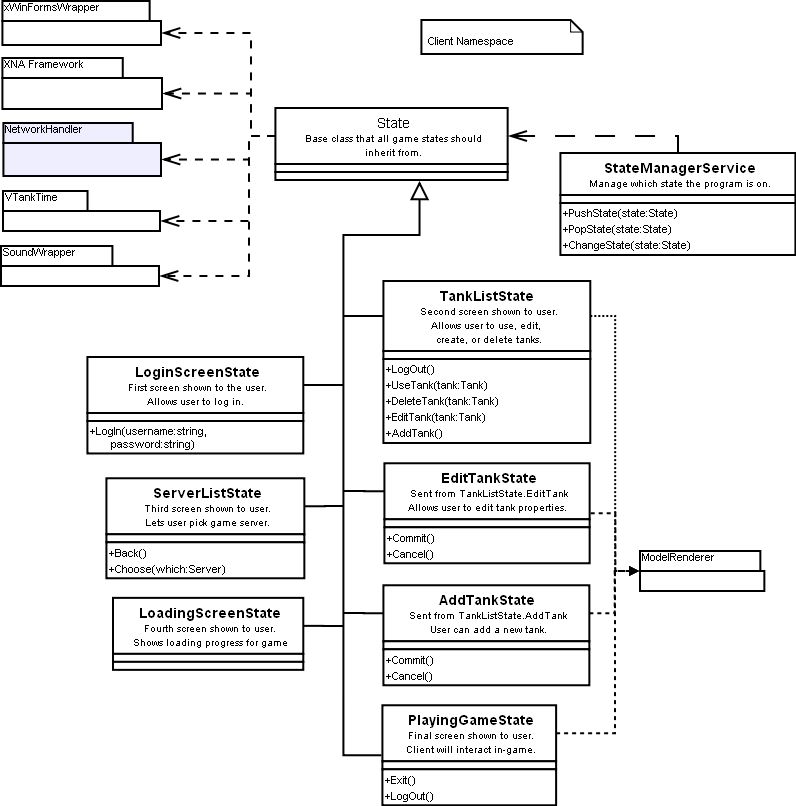
\includegraphics{Figures/Client.png}}
	\caption{\Client UML diagrams}
	\label{fig:clientUML}
\end{figure}

\begin{figure}
	\centering
	\scalebox{0.50}{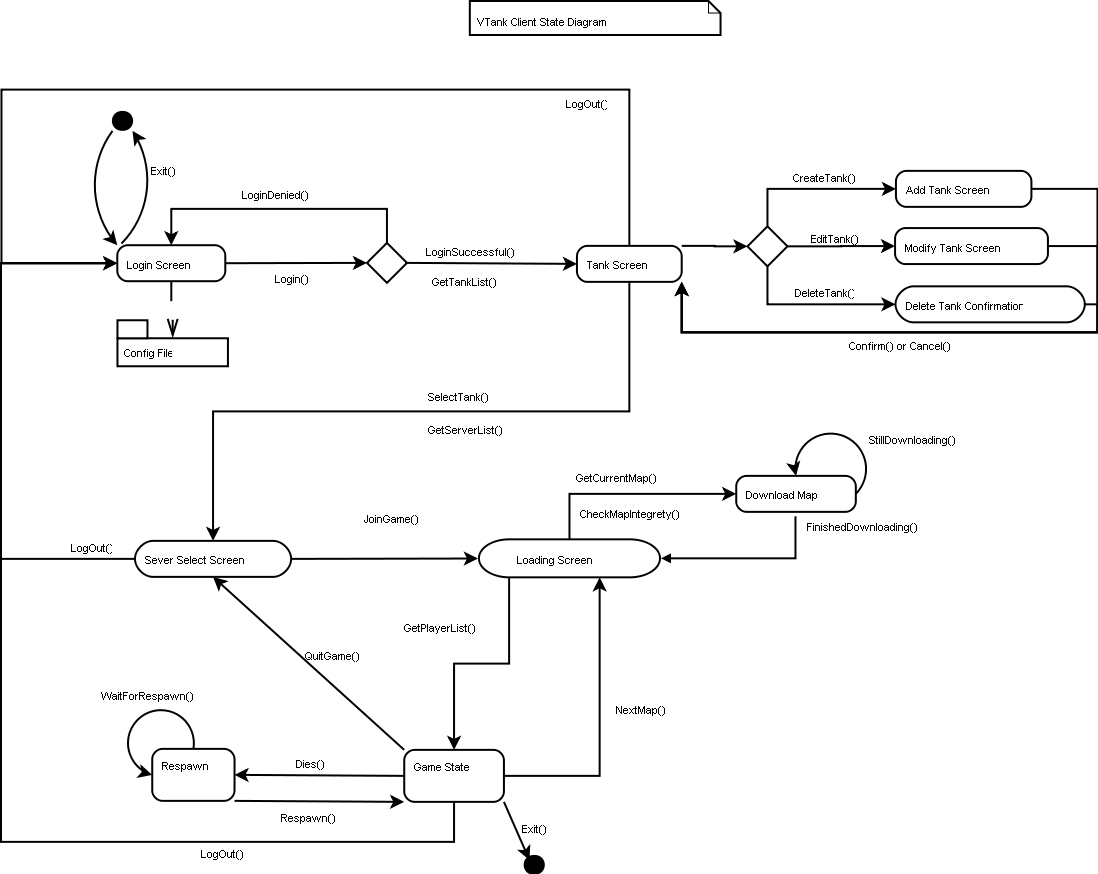
\includegraphics[angle=90]{Figures/ClientStateDiagram.png}}
	\caption{\Client\ state diagrams}
	\label{fig:clientstate}
\end{figure}

\subsection{Renderer}
Renderer is the tool that keeps track of and draws every model and sprite that is seen in the VTank game. Objects in Renderer are called \newterm{entities}. An entity can be a 3D Object, 2D Object, a camera or a light. They all use the same controls to move around in virtual space. Programmers make any object they want to insert into their game an extension of one of the entity classes and then Renderer will take care of moving, animating, and drawing them. 

\begin{center}
\begin{figure}
	\centering
		\scalebox{0.5}{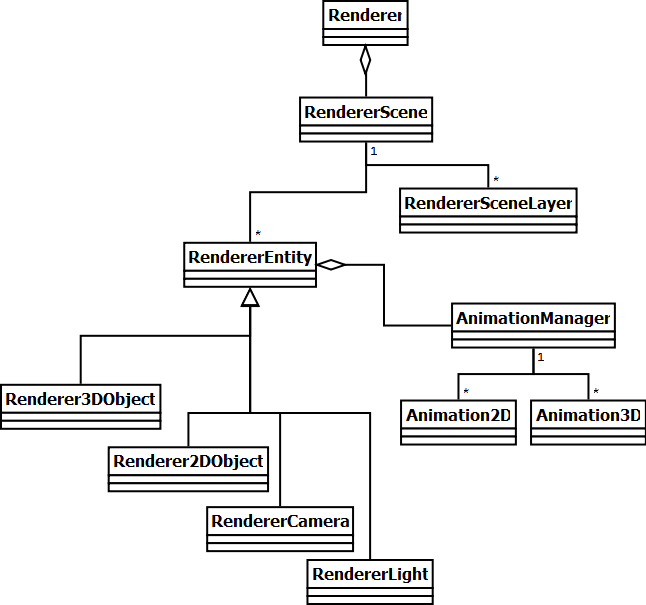
\includegraphics{UML/RendererClassDiagram.png}}
	\label{fig:Renderer Class Diagram}
\end{figure}
\end{center}

\subsection{VTank Networking}

This library will handle all the network operations for our client in a modular way. Such operations include but are not limited to: Connecting to the main server, connecting to a game server, sending a tank's actions, and keeping a connection alive.
  
\subsection{Audio Handler}

The audio handler will control all of the functions relating to storing and playing audio files in the game.

\section{Compiling}

This section assists in compiling \Client\ and all third party tools or libraries used.

\subsection{Windows}

\subsubsection{Building \Client}

\Client\ is a C\# project that uses XNA. Please download and install the following components:

\begin{itemize}
\item Visual Studio 2008 (alternatively, Visual C\# Express works too)
\item Microsoft XNA Framework v\XNAVersion
\item Ice v\IceVersion
\end{itemize}

Once installed, open the \Client\ solution (\filename{Client.sln}) file. Visual Studio will open the project. Build the project from here, and a fresh executable will be compiled.


\section{In-game Interface Components}

\subsection{HUD}

The HUD (Heads Up Display) is composed of two bars that wrap around the user's tank and convey to the user how much health they have and the remaining cooldown on their weapon, respectively.  In the case of special weapons, the cooldown bar may be replaced with a charge-up bar (blue), or an overheat bar (red) for certain weapons. These bars are customizable and scale with the resolution used by the player. It will also dynamically fade in and out based on whether it is being used. 

\begin{figure}[htbp]
	\centering
	\scalebox{0.50}{\includegraphics*{Figures/hud.png}}
	\caption{HUD}
	\label{fig:hud}
\end{figure}

\subsection{Minimap}

The VTank minimap shows a smaller version of what the user can currently see, but with a larger distance on all sides. It displays important information such as enemy/friend locations as well as map objectives such as flags and powerups. It will change to completely transparent if the user passes their mouse over it to avoid hiding an enemy behind it. 

\begin{figure}[htbp]
	\centering
	\scalebox{0.50}{\includegraphics*{Figures/minimap.png}}
	\caption{Minimap}
	\label{fig:mmap}
\end{figure}

\subsection{Scoreboard}

The VTank scoreboard will show the basic statistics for all players in the current game. It is updated in real time and will change formats based on the current type of game being played (DeathMatch, Capture the Flag, etc).  It also displays promotion and team round/game winning messages.

\begin{figure}[htbp]
	\centering
	\scalebox{0.50}{\includegraphics*{Figures/scoreboard.png}}
	\caption{Scoreboard}
	\label{fig:sboard}
\end{figure}

\subsection{Countdown Timer}

A countdown timer in the top left corner of the screen is used to inform players how long they have left before they respawn or when the map is going to change at the end of a game. 

\begin{figure}[htbp]
	\centering
	\scalebox{0.75}{\includegraphics*{Figures/timer.png}}
	\caption{Countdown timers for respawn and map change}
	\label{fig:timer}
\end{figure}

\subsection{\FormWrap Wrapper}

Figure~\ref{fig:formsWrapper}  shows how the client utilizes \FormWrap. A general purpose interface program is wrapped around front of the \FormWrap library to abstract out the creation of these forms. This way, another interface backend can be swapped in, and it will not be necessary to change the GameForm class. For the \FormWrap, the native focus and key/mouse handling support is somewhat lacking, so another layer was necessary to control these actions. The new layer will also be able to read in form configurations through a config files. This allows developers to modify the appearance of their GUI by either hand-modifying these files or through an external forms builder. 
 
\section{\Patcher}

\Patcher\ is the primary interface for the user to configure the client. By clicking the 'Options' button on \Patcher, the program spawns an external client configuration program. This program provides a user-friendly interface for modifying the client's config file, and provides options that affect video performance (resolution, anti-aliasing, fullscreen, refresh rate, quality, etc), audio performance (volume, mute), gameplay (profanity filter, interface options, etc), and input (re-mapping keys, cursor image).

\begin{figure}[htbp]
	\center
	\scalebox{0.75}{\includegraphics*{Figures/patcher.png}}
	\caption{Screenshot of \Patcher\ as of 08/09/2010.}
	\label{fig:launcher}
\end{figure}

Note that the patching functionality of the \Patcher\ is currently disabled.

\section{Particle Effects}

Particle effects are an integral part of the clients presentation method. A particle effect is currently defined by a particle emitter that contains a particle system. Both particle emitter and system can be loaded at runtime from .vtpes (VTank Particle Emitter Settings) and .vtpss (VTank Particle System Setting) files.

In VTank, these files are located in two folder, particleEmitterSettings and particleSystemSettings, that can be found under Client / Driver /Content / resources. To make a new emitter available in game, create a .vtpes and .vtpss file in the correct folders and add them to the Client project. Right click on all added particle files and select 'Properties'. Set 'Build Action' to 'None' and 'Copy to Output Directory' to 'Copy Always'. 
\begin{figure}[h]
	\centering
		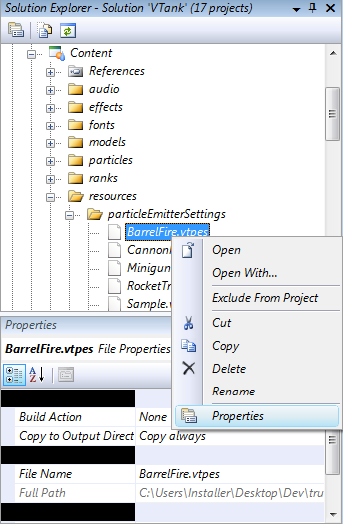
\includegraphics[width=0.50\textwidth]{Figures/AddParticleFiles.png}
	\label{fig:AddParticleFiles}
\end{figure}

Once you've done that the emitter will automatically be loaded into the RendererAssetPool and be available as an emitter. You can create the emitter by calling the ParticleEmitter constructor and passing the name of the file. For example, SuperEmitter.vtpes can be created with the following call:

ParticleEmitter newEmit = new ParticleEmitter("SuperEmitter");

Note that the parameters of a particle emitter setting object can be created dynamically. For example, to change the particle system assiciated with an emitter consider the following.

ParticleEmitterSettings setiings = RendererAssetPool.ParticleEmitterSettings["SuperEmitter"];
settings.ParticleSystemName = "differentSystemName";
ParticleEmitter pemit = new ParticleEmitter(settings);
%%%%%%%%%%%%%%%%%%%%%%%%%%%%%%%%%%%%%%%%%%%%%%%%%%%%%%%%%%%%%%%%%%%%%%%%%%%%
% FILE    : AIFramework.tex
% SUBJECT : Document describing design issues for the VTank AI Framework
% AUTHOR  : (C) Copyright 2009 by Vermont Technical College
%
%%%%%%%%%%%%%%%%%%%%%%%%%%%%%%%%%%%%%%%%%%%%%%%%%%%%%%%%%%%%%%%%%%%%%%%%%%%%

\chapter{\AI}
\label{AI}

\section{Requirements}

\AI\ is a runtime which runs one or more ``bots'' simultaneously. Each ``bot'' is represented by a class in the code which inherits from a bot type known to the framework. This allows programmers to come up with customized implementations of a bot. Implementations of bots are customized by using different logic in certain scenarios. For example, one implementation may respond to being fired at by firing back, while another implementation may decide to run away.

\subsection{Functional Requirements}

A programmer may utilize \AI\ by inheriting from the abstract class \command{VTankBot}. This allows the programmer to override event callbacks sent from the framework. Events are sent to the bot in the following cases:
\begin{itemize}
\item Common update event, sent once per ``tick''. A tick is sent every few milliseconds, as decided by the framework. Note that this event is called even if the bot is dead.
\item A player has joined the game.
\item A player has left the game.
\item A player has entered a chat message.
\item Another player entering a certain radius within the bot. The radius is decided by the framework. It may be the range of the weapon. The bot is considered to have a larger range of sight ahead of it. This radius is referred to as the viewable radius of the bot. This event is ignored if the bot is dead.
\item Another player leaving the viewable radius of the bot. This event is ignored if the bot is dead.
\item The bot has hit a wall. Note that the bot will continue to move forward, but unsuccessfully. The bot should rotate itself out of the wall. This event is called only once per wall collision. If the bot collides with a wall, frees itself, then collides again, only then will it re-send the collision event.
\item A projectile hit another player. Note: The ``player'' may also include the bot itself. This occurs for any projectile event, regardless of who fired. Note that this is the only way the bot can figure out if it's dead or not.
\item A projectile was fired by another player. This does not include the bot itself. This is useful if the bot wants to attempt to dodge the projectile. Note that this event is sent regardless of where the projectile was fired, or who it was fired at.
\item The bot has completed a movement. The bot may ask the framework to move the tank to a certain spot on the map, and the framework's pathfinding will figure out where to go. When this action is done, this event is sent. Part of the event arguments is whether or not the event was successfully completed. For example, if the framework determines that it's impossible to move to the destination, this event will notify the bot of a failure.
\item The bot has completed a rotation. The bot may ask the framework to rotate the tank to a certain degree or to rotate some theta value. When the action is done, this event is sent.
\item A player has respawned. A ``respawn'' is when a player dies, then has waited a specified amount of time, then returns to life. This event is sent regardless of who the player is, including the bot itself. Note that any commands the bot has sent prior to it's death have to be re-sent.
\item The map has rotated. Details on map rotation are available under the \GameServer\ or \Client\ (client) documentation.
\end{itemize}

\subsection{Non-functional Requirements}

\subsubsection*{Platform}

\AI\ is supported for any .NET-supported platform. \AI\ makes extensive use of Ice, so any platform that meets the following requirements may run the framework:
\begin{itemize}
\item The platform supports the .NET 2.0 Framework.
\item The platform supports Ice.
\end{itemize}

\AI\ is currently only officially supported for Windows.

\subsubsection*{Performance}

\AI\ simulates a real client's actions, but unlike a real client, it has no rendering jobs to perform -- it simply performs calculations and logic checks. \AI\ has only a few significant performance requirements:
\begin{itemize}
\item \AI\ must not use 100\% CPU.
\item \AI\ must report events as soon as they happen to each bot being executed; that is, there must be virtually no delay between receiving an event from the game server and sending the event notification to the bot.
\end{itemize}

\subsubsection*{Security}

\AI\ has the same security requirements as the regular client, with one exception: Passwords must be stored somewhere \AI\ can see it, so that it can automatically log into the desired account. It's unreasonable to store the passwords in source code files, so it should be done in external configuration files. \AI\ should automatically encrypt the plain-text password and store the encrypted version instead of the plain-text version. It is acceptable for the account name of the bot to be stored in plain text.

Since the password is sensitive information, the connection to \MainServer\ should use IceSSL. The connection to \GameServer\ may remain unencrypted.

\subsubsection*{User Characteristics}

There are two types of users who should use \AI:
\begin{enumerate}
\item A bot developer who understands a .NET language.
\item A bot runner who manages the configuration files and runs the \AI\ executables.
\end{enumerate}

The user in the former case is expected to be a highly technical user. It's worth mentioning that the programmer does not need to have in-depth knowledge of the \VTank\ protocol; \AI\ will abstract most of the back-end. The programmer's greatest difficulty, then, is proper implementation of intelligent bot programs that can interact with other players.

The user in the latter case does not have to be a technical user whatsoever, assuming that the user has a bot prepared (presumably provided by some other developer). At most, the user would have to inspect configuration files and modify trivial data such as account names and passwords.

\subsubsection*{Scale}

\AI\ is capable of simulatenously executing more than one bot. However, too many bots consume too much CPU and bandwidth. Because \AI\ exists to provide human players with things to shoot at (as opposed to human players joining an empty server and being bored), \AI\ is not required to have high scalability in regards to number of players. A reasonable number of bots, then, is considered to be 4. \AI\ can possibly support more than 4 simultaneous bots, but does not necessarily need to.

\subsubsection*{Data Formats}

The only external data relevant to programmers or users of \AI\ is the configuration file. The configuration file uses the formatting required for Ice configuration files, which holds the following format:

\begin{command}
key = value
\end{command}

\AI\ reads the configuration file upon start-up for Ice configuration and for username and password information. This is stored in the following way:

\begin{command}
ClassName = username:password
\end{command}

\command{ClassName} represents the name of the bot class. For example, if one defines a bot using the syntax, \command{class MyBot}, the key for this property would be ``MyBot''. On the right-side of the equal sign, the username is stored first, followed by a colon (which acts as the delimiter), followed by the password, which can be any number of characters of any type. After running \AI\ once, \AI\ will automatically read the password in, encrypt the password, and store the encrypted version. This is denoted by an exclamation mark as the delimiter instead of a colon. For example, this is a bot whose password is encrypted:

\begin{command}
ClassName = username!encryptedPassword
\end{command}

Note that attempting to insert an exclamation mark with an unencrypted password may result in an undefined error or an incorrect password.

\subsubsection*{Internationalization}

\AI\ documentation, class names, methods, and namespaces are written in US English. There are currently no plans to port \AI\ to a different language. However, it's not unreasonable for programmers to write bots in different languages.

%%%%%%%%%%%%%%%%%%%%%%%%%%%%%%%%%%%%%%%%%%%%%%%%%%%%%%%%%%%%%%%%%%%%%%%%%%%%
% FILE    : WeaponSystem.tex
% SUBJECT : Document describing the VTank weapon system, and its XML based
% specification system for weapons and projectiles.
% AUTHOR  : (C) Copyright 2010 by Vermont Technical College
%
%%%%%%%%%%%%%%%%%%%%%%%%%%%%%%%%%%%%%%%%%%%%%%%%%%%%%%%%%%%%%%%%%%%%%%%%%%%%

\chapter{Weapon System}
\label{Weapon System}

\section{Introduction}
VTank's weapon system was created in an effort to streamline the addition of new weapons into the game.  The goal of the weapon system is to minimize weapon-specific coding for primary weapons, in order to allow for the addition of a myriad of new weapons, with virtually no coding required.  

\section{XML Specification Properties}
The VTank weapon specification markup follows a similar format for weapons, projectiles, and environmental effects.  There are three files that describe all of these for VTank, \WeapProps\, \ProjProps\, and \EnvProps\, each encapsulating multiple weapons or projectiles or environmental effects.  The convention this document will use for describing these properties is:

\begin{description}
\item \command{<propertyName>} (number required)  Description of the property.
\end{description}

Required properties (1) that are children of optional properties (0-1 or 0-*) are not required in the absence of their parent properties. 

\subsection{Weapon Properties}
\begin{description}
\item \command{<Weapon Properties>} (1) The root element in \WeapProps\ that describes the entire collection of weapons.  Nothing in \WeapProps\ should be outside of the ending and closing tag of this element. 

\item \command{<weapon>} (0-*) Encapsulates an entry for a single weapon.  Will have many optional/mandatory entries describing the weapon.

\item \command{<id>} (1) The ID of this weapon.  Should be unique and incrementing in accordance with other weapon entries.

\item \command{<name>} (1) The name of this weapon.

\item \command{<weaponFireSound>} (0-1)  The sound this weapon produces when fired.

\item \command{<weaponChargingSound>} (0-1)  The sounds this weapon makes when charging up.  

\item \command{<model>} (1) The name of the model associated with this weapon.

\item \command{<deadModel>} (0-1)  The name of the dead version of this model, for usage when the tank is destroyed.  

\item \command{<muzzleEffectName>} (0-1)  The name of the muzzle flash particle effect associated with this weapon.  

\item \command{<customColor>} (0-1)  Indicates that the weapon uses a custom color, rather than the default. (The tank's color.)

\item \command{<colorMesh>} (0-1)  The model mesh that color should be applied to ingame.

\item \command{<emitters>} (0-1) Encapsulates a collection of zero or more emitters.  Emitters are used as mount points for particle effects ingame.
\item \command{<emitter>} (0-*)  A child of the emitters element, representing a single emitter.  Describes a point that may host particle effects 
\item \command{<emitterName>} (1) The name of a given emitter.  The name given will be used as a reference for the attachment of particle effects ingame.
\item \command{<effectName>} (1)  The particle effect associated with this emitter.

\item \command{<animations>} (0-1)  Encapsulates a collection of zero or more animations.  While models only contain one track of animation, specific sets of frams may make up a single animation.
\item \command{<animation>} (0-*)  A child of the emitters element, representing a single animation contained in the model.
\item \command{<name>} (1)  The name of this animation.  By convention 'still' indicates that the starting/ending frame is the resting state of the model, to be played constantly (if applicable).  'firing' indicates the animation to be played when the weapon fires.
\item \command{<startingFrame>} (1)  The frame where this animation starts.
\item \command{<endingFrame>} (1)  The frame where this animation ends.
\item \command{<handlerClass>} (1)  The class that handles the playing of this animation.  

\item \command{<projectileID>} (1)  The id associated with the projectile this weapon fires.
\item \command{<cooldown>} (1)  The cooldown of this weapon, I.E. the delay between each shot.
\item \command{<launchAngle>} (0-1)  The angle that this weapon fires at.  If absent or left blank, implies an angle of 0 degrees, or parallel to the ground.
\item \command{<maxChargeTime>} (0-1)  The time required to charge this weapon to its maximum damage.
\item \command{<projectilesPerShot>} (0-1)  The number of projectiles launched each time the weapon is fired.  If absent or left blank, it implies one projectile.
\item \command{<intervalBetweenEachProjectile>} (0-1)  The delay between each projectile, for usage with weapons that fire multiple projectiles.  Should not be used unless using multiple projectiles per shot.
\item \command{<overheatTime>} (0-1)  The time it takes for this weapon to overheat.  Absent or blank for no overheating.
\item \command{<overheatAmountPerShot>} (0-1) The amount (as a percentage) that each shot overheats the weapon.  Overrides \command{<overheatTime>} if present  Absent or blank for no overheating.  
\item \command{<overheatRecoverySpeed>} (0-1) The speed that this weapon recovers at, as a floating point value to be multiplied against delta time (time between frames).  1.0 indicates normal recovery speed, while 2.0 would be 2x speed.
\item \command{<overHeatRecoverStartTime>} (0-1)  The interval between firing and recovery.  If absent or blank when overheating is specified, implies that recovery starts immediately.
\end{description}

\subsection{Projectile Properties}

\begin{description}
\item \command{<projectileProperties>} (1)  The parent element of the \ProjProps\ file.  Nothing should be outside of this tag.
\item \command{<id>} (1)  The ID of this projectile.  Should be unique and increment relative to other entries.
\item \command{<name>} (1) The name of this projectile.
\item \command{<modelName>} (0-1)  The name of the model associated with this projectile.  If left blank, implies that only the particle effect listed under particleEffectName will be used to represent the particle. 
\item \command{<scale>} (0-1)  The scale of this projectile.  If left absent or blank, implies a scale of 1.0 (normal).
\item \command{<particleEffectName>} (0-1)  The name of the particle effect associated with this projectile.  If this element coexists with modelName, this particle effect will emanate from the model.
\item \command{<impactParticleName>} (0-1)  The particle effect to be triggered when the projectile impacts with a collidable or damageable object.
\item \command{<expirationParticleName>} (0-1)  The particle effect to be triggered when the projectile expires (reaches its max range).

\item \command{<emitters>} (0-1) Encapsulates a collection of zero or more emitters.  Emitters are used as mount points for particle effects ingame.
\item \command{<emitter>} (0-*)  A child of the emitters element, representing a single emitter.  Describes a point that may host particle effects 
\item \command{<emitterName>} (1) The name of a given emitter.  The name given will be used as a reference for the attachment of particle effects ingame.
\item \command{<effectName>} (1)  The particle effect associated with this emitter.

\item \command{<animations>} (0-1)  Encapsulates a collection of zero or more animations.  While models only contain one track of animation, specific sets of frams may make up a single animation.
\item \command{<animation>} (0-*)  A child of the emitters element, representing a single animation contained in the model.
\item \command{<name>} (1)  The name of this animation.  By convention 'still' indicates that the starting/ending frame is the resting state of the model, to be played constantly (if applicable).  'firing' indicates the animation to be played when the weapon fires.
\item \command{<startingFrame>} (1)  The frame where this animation starts.
\item \command{<endingFrame>} (1)  The frame where this animation ends.
\item \command{<handlerClass>} (1)  The class that handles the playing of this animation.  
\item \command{<areaOfEffectRadius>} (0-1)  Indicates the radius of the projectile's area of effect damage.  If this element coexists with areaOfEffectUsesCone, this field indicates the width of the distant end of the cone.
\item \command{<areaOfEffectUsesCone>} (0-1)  Indicates whether the areaOfEffect for this projectile should take a cone shape (triangle in reality).  If using a cone, the areaOfEffectRadius will become the length of the far side of the triangle, while the height of the triangle will be formed by the range of the weapon. 
\item \command{<areaOfEffectDecay>} (0-1)  Defines the the damage at the edge of the AoE radius as a percentage of the whole. 1.0 indicates 100\%, where .5 indicates 50\%.  If absent or left blank, implies full damage inside the AoE radius.
\item \command{<coneRadius>} (0-1)  The radius of a cone used to produce weapon scatter.  Much like the AoE cone, this triangle is formed by taking this radius as the far width of the triangle (bottom), and the range as the height.  If this property is specified, projectiles will deviate randomly within this cone when fired.
\item \command{<coneOriginWidth>} (0-1)  When using areaOfEffectUsesCone, defines the width of the origin of the cone in pixels.  Using an origin larger than 0 will produce a quadrilateral instead of a triangle.  If left blank or absent, implies a width of 0, if used without areaOfEffectUsesCone
\item \command{<coneDamagesEntireArea>} (0-1)  Relevant when areaOfEffectUsesCone is specified, this property explicitly states that the entire area of the cone will receive damage.  Useful for weapons that emit point blank damage to a region in front of or around them.
\item \command{<minDamage>} (1)  The minimum damage this weapon will inflict, where the damage a weapon inflicts is a random value between the min and max damage.
\item \command{<maxDamage>} (1)  The maximum damage this weapon will inflict.
\item \command{<isInstantaneous>} (0-1)  Indicates whether this projectile has a flight time.  Nullfies all velocity/accelleration related fields if used.
\item \command{<initialVelocity>} (0-1)  Velocity in pixels per second that this projectile will be moving at the moment it is fired.
\item \command{<terminalVelocity>} (0-1)  Velocity that this projectile will accelerate to.
\item \command{<acceleration>} (0-1)  The acceleration in pixels per second that this projectile will accelerate.
\item \command{<range>} (0-1)  The range of this projectile (in pixels).
\item \command{<rangeVariation>} (0-1)  The variation in pixels that this projectile may end at.  Given a variation, the projectile will expire/land at a random point within range +/- rangeVaration.
\item \command{<jumpRange>} (0-1)  The range within which this projectile may 'jump' to deal additional damage. (Chain Lightning effect)
\item \command{<jumpDamageDecay>} (0-1)  The reduction in damage applied at each damage jump.
\item \command{<jumpCount>} (0-1)  The number of times this projectile may jump.
\item \command{<environmentEffectID>} (0-1)  The id of any environment effect associated with this projectile.  This may include things such as burn marks, or fires left on the ground.
\end{description}
\subsection{Environment Properties}

\begin{description}
\item \command{<EnvironmentProperties>} (1)  The parent element of \EnvProps\ encapsulates zero or more environmental effects that trigger from projectiles.
\item \command{<environmentProperty>} (0-*)  A single environmental effect entry.
\item \command{<id>} (1)  The id of this environment effect, should be unique and incrementing.
\item \command{<name>} (1)  The name of this environment effect.
\item \command{<triggersUponImpactWithEnvironment>} (0-1)  Indicates whether this effect triggers when it impacts with a collidable or damagable object.
\item \command{<triggersUponImpactWithPlayer>} (0-1)  Indicates whether this effect triggers when it impacts with a player.
\item \command{<triggersUponExpiration>} (0-1) Indicates whether this effect triggers when the projectile expires.
\item \command{<particleEffect>} (1)  The particle effect associated with this environmental effect.
\item \command{<duration>} (0-1)  The duration of this environmental effect.
\item \command{<interval>} (0-1)  The interval between damage applications, for environmental effects that damage players.
\item \command{<areaOfEffectRadius>} (0-1)  The radius of the circle that this effect influences.
\item \command{<areaOfEffectDecay>} (0-1)  Like projectile's AoE decay, specifies the damage at the edge of the radius, as a floating point percentage of damagePerInterval.
\item \command{<minDamage>} (0-1)  The minimum damage this effect will deal per tick (at each interval).
\item \command{<maxDamage>} (0-1)  The maximum damage this effect will deal per tick.
\end{description}
%%%%%%%%%%%%%%%%%%%%%%%%%%%%%%%%%%%%%%%%%%%%%%%%%%%%%%%%%%%%%%%%%%%%%%%%%%%%
% FILE    : MapEditor.tex
% SUBJECT : Document describing design issues in the VTank Map Editor.
% AUTHOR  : (C) Copyright 2010 by Vermont Technical College
%
%%%%%%%%%%%%%%%%%%%%%%%%%%%%%%%%%%%%%%%%%%%%%%%%%%%%%%%%%%%%%%%%%%%%%%%%%%%%

\chapter{\MapEditor}
\label{mapeditor}

\section{Requirements}

\MapEditor\ is the \VTank\ map editor. \VTank\ is an overhead shooting game played on different maps. Each map has an objective such as capture the flag, king of the hill, or death match. Each map will be large enough to support many users and therefore can be larger than a single screen. As the player moves his or her tank, the screen will scroll along the map, keeping the tank centered as much as possible. In order to make the maps a map editor is needed. This section describes that editor.

\subsection{Functional Requirements}

\MapEditor\ will be used to create maps to be used within the \VTank\ game. \MapEditor\ must be able to create a map, load a map, modify a map, and save a map both to and from  a \filename{*.vtmap} file and directly to and from \MainServer\ (where the actual maps being used are stored). Each map thus has a ``home location'' either in a disk file or on the server. Whenever a map is saved it is saved back to its home location.

Maps are composed of tiles that define a coordinate system for the map. Each map contains information about the map's dimensions (in tiles), along with tile data for each tile. Every tile has seven things associated with it. They are as follows:
\newpage
\begin{itemize}
\item A tile id
\item An object id
\item A event id
\item A flag stating the collision
\item A height (also in tiles)
\item A type 
\item An effect 
\end{itemize}

The tile id field is used to store an integer that corresponds to a graphical image which will appear as the tile background to the user. The object id and event id fields will work every similar by storing integers that correspond to events and objects that can be placed on top of the tile background. The collision flag is used to set whether or not a tank can drive through the tile. Height will be used to give the tile height it will be set in terms of tiles. The type field will be used to determine if a tile is land or water and effect field will be used if a particular tile background should have an effect on the tank (ex. Mud slowing down the tank speed). For a more technical explaination of the tile format see Map File Format.

Tiles can have two types of collision, implicit and explicit. Implicit collision is where projectiles and tanks can't pass through the tile due to the tile having height. It's `implicit' because the map editor does not (have to) manually set the collision for this tile: it's implied that a tile with a height greater than zero cannot be passable. Explicit collision is where only tanks can't pass through. There are some tiles that have a height of zero but are still not passable (such as water). Explicit collision, then, allows projectiles to pass over the tile.

\subsubsection{Tile Layers}

Maps are composed of layers. There are three basic layers that make up each \VTank\ map:
\begin{itemize}
\item The Terrain Layer
\item The Object Layer
\item The Event Layer
\end{itemize}
The terrain layer will be the basis of any tile. It will be composed of a graphic image that creates the "background" of a tile. The terrain layer will be represented with a green box icon as shown in the tools section.

The object layer will be for displaying static objects on tiles. Static objects are things such as barrels, bushes, rocks, etc. These objects will be placed on top of any existing terrain. The object layer will be represented with a blue box icon as shown in the tools section.

The event layer will be used for storing spawn points and other events such as flag spawns and captures. These events will be represented by different images in \MapEditor,\ but won't be visible during game play. The event layer will be represented by a yellow box icon as shown in the tools section. Below is a table of the current events that make use of this layer.

\begin{center}
\centering
\begin{tabular}{ | c | p{8cm} |}
\hline
Event 	& Description \\	[1.0ex]
%heading
\hline\hline
Player Spawn Point 	& The player spawn point is where a player's tank will start in the map when the game starts or where they will start from after dying. This event will be needed in all maps. \\	[1.0ex]
Team Spawn Area 	&	The team spawn area is where teams will start in the map when the game starts or where individuals of that team will start from after dying. This means each team needs their own team spawn area. Team spawn areas will be needed for team game modes. \\	[1.0ex]
Flag Spawn Point 	& The Flag spawn point is where a flag will start in the map when the game starts or where the flag will return to after it has been reset. It will also double as the flag caputure point for where the enemy flag must be brought to in order to score. Flag spawn points are needed in the capture the flag game mode. \\	[1.0ex]
King of the Hill Area		& King of the hill area is used in the King of the hill game mode. This area represents the hill where the player's tank must be in order to score points in king of the hill. \\  [1.0ex]
\hline\hline
\end{tabular}
\label{table:nonlin}
\end{center}


\subsubsection{Map File Format}

The map editor must save the map data in a specific way. In the same way that it was saved, the map file will be read into memory. Other modules in different languages may implement their own version of the module which reads in or saves maps in \MapEditor. The class responsible for loading/saving the map file must follow this exact format:

\emph{Line 1}: 
\begin{itemize}
	\item Version byte [1 Byte]: Version of the map. Should increment every time the format of the map changes.
	\item Title [n Bytes]: String value that holds the name of the map.
\end{itemize}
\emph{Line 2}: 
\begin{itemize}
	\item Width of the map [4 Bytes]: Number of tiles horizontally. The value is always greater than zero and is stored in binary format.
	\item Height of the map [4 Bytes]: Number of tiles vertically. The value is always greater than zero and is stored in binary format.
	\item Supported game modes [N Bytes]: Each game mode is a single byte-form integer between 0 and 255 (except for 12). The entire line is reserved for game mode flags, so as many game modes as are available are supported. \emph{The map module must not allow 0x0A as a possible flag}. The 0x0A byte is reserved for the newline character.
\end{itemize}
\emph{Line 3+}: List of tiles. There should be exactly MapWidth x MapHeight tiles. Each tile follows this exact format:
\begin{itemize}
	\item Tile ID [4 Bytes]: The ID of the tile in binary format. Convert the 4 bytes to it's integer form in little-endian order (the first significant byte is on the left). This field represents the terrain layer of the map.
	\item Object ID [2 Bytes]: The ID of the object that sits on this tile in binary format. Convert the 2 bytes into it's integer form in little-endian order (the first significant byte is on the left). If both bytes are 0x00 (i.e. if the object ID is zero), that is symbolic for no object on this tile. This field represents the object layer of the map.
	\item Event ID [2 Bytes]: The ID of the ``event'' that sits on this tile. Convert the 2 bytes to it's integer form in little-endian order (the first significant byte is on the left). This field represents the event layer of the map.
	\item Tile collision [1 Byte]: A boolean value in binary format. The 0x00 byte means that the tile is not passable (by tanks). Any other byte means that the tile is passable (by tanks).
	\item Tile height [1 Byte]: An integer value in binary format. The value is between 0 and 255 and can be converted to it's integer form with a simple cast.
	\item Terrain type [1 Byte]: Type of terrain in binary format. The value is between 0 and 255. This field is reserved for future implementation.
	\item Tile effect [1 Byte]: Effect of the tile in binary format. This value is between 0 and 255. This field is reserved for future implementation. This field will contain information about how a tile can affect a player's movement.
\end{itemize}

The total size of each tile is 12 bytes. The file size (in bytes) of each map file can be calculated like this:

\begin{commands}
Length of title + number of game modes supported + (number of tiles * 12) + 11
\end{commands}

\subsubsection{Game Modes}

The following game modes are supported:
\begin{center}
\centering
\begin{tabular}{ | c | c | c | p{8cm} |}
\hline
ID 	& Mode Name					& Teams 		& Description \\	[1.0ex]
%heading
\hline\hline
0 	& Deathmatch 				& No 				& Deathmatch is a straight free-for-all kill-fest between every tank and every other tank. The player spawns at spawn points defined in the event layer randomly. \\	[1.0ex]
1 	&	Team Deathmatch 	& Yes				& Team Deathmatch is a team free-for-all kill-fest between two or more teams. The objective is to have more kills than the other teams. Players spawn together in a team spawn area defined in the event layer. \\	[1.0ex]
2 	& Capture the Flag  & Yes				& Capture the Flag pits two teams against each other with the objective of capturing the other player's flag and returning it to their own base. If a player is killed while holding the flag, the flag is dropped on the ground.  The team who owns the flag can run over it to return it to the base instantly, while the team who is trying to capture the flag can run over it to pick it up and continue running it home. \\	[1.0ex]
3		& King of the Hill	& Sometimes	& King of the Hill invites every player to attempt to conquer and maintain control of an objective  for the longest period of time. When one player or team has control of the  objective, their score increments. At the end of the round, the player or team with the highest score wins the game. \\  [1.0ex]
\hline\hline
\end{tabular}
\label{table:nonlin}
\end{center}

\newpage

\subsubsection{Tools}

\MapEditor\ will provide its users with a varity of tools for editing the maps. The following user interface mock-up shows the intended layout of \MapEditor.\  Figure~\ref{fig:map-editor} shows the basic layout of \MapEditor's\ tools and controls.

\begin{figure}[htbp]
  \centering
  \scalebox{0.5}{\includegraphics*{Figures/mapeditormain.png}}
  \caption{Gardener's Main Screen}
  \label{fig:map-editor}
\end{figure}
\begin{table}[]
\caption{Tools of \MapEditor\ }
\begin{tabular}{| c | p{12cm} |}
\hline\hline
Icon & Description \\ [0.5ex]
\hline 
\includegraphics*{Figures/newmap.png} & This button brings up the new map dialog that
																				allows the user to create a new map.\\	[1.0ex]
\includegraphics*{Figures/open.png} & This button allows the user to select a map and
																			then open it.\\	[1.0ex]
\includegraphics*{Figures/saveas.png} & This button allows the user to save the current
																				map open under a new name.\\	[1.0ex]
\includegraphics*{Figures/save.png} & This button allows the user to save the current 
																			map open.\\	[1.0ex]
\includegraphics*{Figures/server.png} & This button opens the server dialog that allows
																			the user to upload, download, remove and view the 
																			maps. \\	[1.0ex]
\includegraphics*{Figures/mapprop.png} & This button displays the current map's properties. \\																																			  [1.0ex]
\includegraphics*{Figures/gamemodes.png} & This button allow the user to set game modes for 
																			the loaded map \\ [1.0ex]
\includegraphics*{Figures/terrainlayer.png} & This button allows the user to work on the 																																							terrain layer. \\	[1.0ex]
\includegraphics*{Figures/objectlayer.png} & This button allows the user to work on the object 																						 														layer. \\	[1.0ex]
\includegraphics*{Figures/eventlayer.png} & This button allows the user to work on the event 																																					layer. \\	[1.0ex]
\includegraphics*{Figures/cut.png} & This buttton allows the user to cut tiles out of the map \\	[1.0ex]
\includegraphics*{Figures/copy.png} & This button allows the user to copy tiles from the map. \\	[1.0ex]
\includegraphics*{Figures/paste.png} & This button allows the user to paste tiles previously cut or copied\\	[1.0ex]
\includegraphics*{Figures/pointer.png} & This button allows the user to draw tiles, tile by tile. \\ [1.0ex]
\includegraphics*{Figures/fill.png} & This button allows the user to fill selected tiles with a 																																			selected graphic. \\	[1.0ex]
\includegraphics*{Figures/selectgrp.png} & This button allows the user to select multiple tiles. 																				 															\\	[1.0ex]
\includegraphics*{Figures/fillgrp.png} & This button allows the user to draw tiles, multiple at a time. \\																				 																[1.0ex]
\includegraphics*{Figures/gridtoggle.png} & This button allows for the grid to be toggled on or 																																			off. \\	[1.0ex]
\includegraphics*{Figures/collisiontoggle.png} & This button allows for the collision to be 																									 												toggled on or off. \\	[1.0ex]
\includegraphics*{Figures/heighttoggle.png} & This button allows for the height indicators to be toggled on or off. \\	[1.0ex]
\hline %inserts single line
\end{tabular}
\end{table}
\newpage

\subsection{Adding Content}

\MapEditor\ uses a variety of different content, mostly images to create the overall map. This section gives a brief explanation on how to add additional content to \MapEditor\ while were in production.

Terrain, Event, and Object images all work the same way in \MapEditor,\ therefore adding them to \MapEditor\ works the same also. Images for terrains, objects or events all have to be 64 x 64 pixels, because that is the standard tile size of the tiles that make up maps. The images in general go in the VTank/Map\_Editor/data/ folder then in the appropriate subfolder for terrain, objects, or events.

After the images have been added, \MapEditor\ has to know of their existence. This is where the dictionaries come in to play. There are three separate dictionaries, one for terrain, objects, and events. Therefore the user adding content must open the appropriate dictionary for the images he or she added. Dictionaries can be found in the VTank/Map\_Editor folder. Next the user must read the directions at the top of the dictionary for how to add the images to the dictionary. These directions will explain the format for adding the images. Then when ready scroll to the bottom and add the images. 

*Note: If adding terrain images to Gardener, in order for them to be rendered properly in game, copy the tiles into: VTank/Client/Driver/Content/textures/tiles/, and copy tiles\_dictionary.txt into VTank/Client/Driver/. Also in Visual Studio in the VTank solution, expand the Client project, right-click on Content->textures->misc->tiles, click 'Add existing item...', then highlight all of the new tiles to add them to the client content project.

\subsection{Use Cases}

The following case allows the user to edit an existing map.

\begin{usecase}
  {OPEN MAP}
  {Editing User}
  {\MapEditor\ is running and the user wishes to edit an existing map.}
\begin{enumerate}
\item User makes appropriate menu selection.
\item Dialog box prompts user for the name of the map to edit. This includes the map's ``home'' (a disk file or from the server).
\item The map is loaded. It is an error if the map does not yet exist.
\end{enumerate}
\end{usecase}

The following case allows the user to create a new map. This is different than the OPEN MAP case because when a new map is being created certain bits of initial information must be provided. In contrast when an existing map is being edited that information is part of the map and does not need to be specified by the user.

\begin{usecase}
  {NEW MAP}
  {Editing User}
  {\MapEditor\ is running and the user wishes to edit a new map.}
\begin{enumerate}
\item User makes appropriate menu selection.
\item Dialog box prompts user for attributes of the new map. This includes the map's home (a disk file or from the server).
\item A blank map is loaded. It is an error if the map already exists.
\end{enumerate}
\end{usecase}

The following case allows the user to modify the attributes of an existing map. These are the same attributes that are provide when a new map is created.

\begin{usecase}
  {CHANGE MAP ATTRIBUTES}
  {Editing User}
  {\MapEditor\ is running with a map loaded and the user wishes to modify the attributes of the map.}
\begin{enumerate}
\item User makes appropriate menu selection.
\item Dialog box prompts user for new attributes of the map. This includes the map's home (a disk file or from the server).
\item If possible the attributes are changed. If the map's home is changed, it is removed from its old home (after being saved to its new home).
\end{enumerate}
\end{usecase}

The following case allows the map to be saved to its home or to a different file.

\begin{usecase}
  {SAVE MAP}
  {Editing User}
  {\MapEditor\ is running with at least one map loaded and the user wishes to save that map.}
\begin{enumerate}
\item User makes appropriate menu selection.
\item If the user simply selects `Save' the current map is saved to its home location (either in a file or on the server). If the user selects `Save As' the user is prompted for a new file into which to save the map. This does not change the current map's home location, however.
\end{enumerate}
\end{usecase}

The following case allows the user to manage the tiles database.

\begin{usecase}
  {MANAGE TILES}
  {Editing User}
  {\MapEditor\ is running. It is not necessary for any maps to be loaded.}
\begin{enumerate}
\item User makes appropriate menu selection.
\item Dialog box appears that allows the user to perform various operations on the local tile database.
  \begin{enumerate}
    \item Display tile IDs and descriptions.
    \item Change graphic image associated with a tile ID.
  \end{enumerate}
\end{enumerate}
\end{usecase}

\pcnote{We still need use cases for editing maps!}

\subsection{Non-Functional Requirements}

\subsubsection*{Platform}

\MapEditor must support both Windows and Linux. It must be a GUI application with a reasonably native look and feel on each platform. Future support for the Mac OS X operating system is also possible.

\subsubsection*{Performance}

\MapEditor\ should be able to load and save maps in a time that is acceptable to an interactive user (a few seconds at most). It should be responsive to the user with no perceptible delay during in reacting to most commands. When editing a large map the bulk of the memory consumption should be due to a single copy of the map data itself.

\subsubsection*{Security}

\MapEditor\ should keep the user's ID and password on the main server secure. It should not store this information in a file nor transmit it over the network unencrypted. \MapEditor\ should protect itself from malicious maps and servers. For example, editing a map downloaded from an untrusted web site or from an untrusted \VTank\ server should be safe.

\subsubsection*{User Characteristics}

It can be assumed that the users of \MapEditor\ are competent computer users but they are not programmers or computer specialists. It can be assumed that they are familiar with the platform on which the map editor is running and that they will expect \MapEditor\ to behave according to the established standards for that platform. For example shortcut key combinations should be as expected for the platform.

\subsubsection*{Scale}

\MapEditor\ needs to be able to handle maps of arbitrary size since users may wish to create very large maps. It only needs to support a single user at a time. Furthermore it can be assumed that no other program is editing or using a map while \MapEditor\ is in control of it.

Note that it is acceptable to limit the size of a map to that which can be conveniently held in memory. It is not necessary for \MapEditor\ to swap map data between memory and disk while the map is being edited. As a practical matter this will limit the size of a map to 2 GiB or less (on 32 bit systems).

\subsubsection*{Data Formats}

\MapEditor\ must read and write map files in the \VTank\ specific \filename{*.vtmap} format (the precise nature of which is left unspecified). \MapEditor\ must support tile images in at least \filename{*.png} format, but support for other tile image formats is encouraged.

\subsubsection*{Internationalization}

Initially \MapEditor\ only needs to support US English. Support for other languages and cultures is not required\footnote{Except for Latin, of course.} but may be a future enhancement.

\section{Compiling}

\MapEditor\ is supported on the following platforms. It is known to compile and work on these platforms although it may also work on variations of these platforms or closely related platforms.

\begin{itemize}
\item Windows XP with Microsoft Visual Studio 2008 (Visual C++ v9.0)
\item openSUSE Linux 11.1 with Code::Blocks v8.02 (g++)
\end{itemize}

The following paragraphs describe how to set up \MapEditor\ for development on these platforms. Note that if you are a user of \MapEditor, you do not need to read this section.

\subsection{Windows}

\subsubsection{Building the \MapEditor}

Once you have the prerequisite libraries in place, you are ready to build \MapEditor. Load the \filename{Map\_Editor.sln} file into Visual Studio. Notice that two configurations have been defined. The Release configuration builds an optimized version of \MapEditor\ suitable for distribution. The Debug configuration builds a debugging version for use during testing. In general you should use the debug version during development since certain run time checks (assertions, memory leak detection, etc) have been enabled only in that version.

In addition to the main project for the map editor itself, the Visual Studio solution file also contains a project for \MapEditor\ unit tests. This project is named the ``check'' project. If you build the entire solution, the check project is also built.

Use Visual Studio to build the configuration(s) you desire. Executable files are placed in their respective output folders. Note that the executables should be run from the \MapEditor\ root folder since otherwise they will not be able to locate their data resources in the data folder. The unit test executables can be run separately from \MapEditor and should be exercised before \MapEditor\ is used to verify that there are no problems with the \MapEditor's internal components.

\subsubsection{Precompiled Headers}

\MapEditor\ has been organized to take advantage of precompiled headers. Specifically the header \filename{Library.hpp} contains include directives for all C++ standard library headers and for headers from third party libraries such as wxWidgets. Each source file in the map editor includes \filename{Library.hpp} as the first header included. Map editor specific headers follow \filename{Library.hpp} as necessary. This means that every source file in the map editor sees the library environment in exactly the same was as every other source file. This promotes consistency and simplifies header management. Ironically it can also improve compilation speed by allowing the compiler to precompile the \filename{Library.hpp} header. The source file \filename{Library.cpp} exists only to manage this precompilation. \filename{Library.cpp} is not otherwise used by \MapEditor\ code.

\subsection{Linux}

The official way to build \MapEditor\ on Linux is to use Code::Blocks. Although not currently provided, you could also create a Makefile for \MapEditor\ and use it to build the program. This option is not discussed further here.

We recommend that you build Code::Blocks from source. Compiling Code::Blocks is straightforward once you have wxWidgets compiled and installed. Download and unpack v8.02 and follow the (simple) instructions included.

To actually build \MapEditor\ load the \filename{Map\_Editor.cbp} file into Code::Blocks and select the build option.

%%%%%%%%%%%%%%%%%%%%%%%%%%%%%%%%%%%%%%%%%%%%%%%%%%%%%%%%%%%%%%%%%%%%%%%%%%%%
% FILE    : CaptainVTank.tex
% SUBJECT : Document describing design issues in Captain VTank.
% AUTHOR  : (C) Copyright 2009 by Vermont Technical College
%
%%%%%%%%%%%%%%%%%%%%%%%%%%%%%%%%%%%%%%%%%%%%%%%%%%%%%%%%%%%%%%%%%%%%%%%%%%%%

\chapter{Captain \VTank}
\label{captainvtank}

\section{Requirements}

Captain \VTank\ is the administrative client for \VTank. Captain \VTank\ authenticates with \MainServer\ to perform high-level operations, including stopping, starting, or restarting \MainServer, managing user accounts, managing online users, managing instances of the \GameServer, monitoring server health, kicking online users, banning or suspending online or offline users, creating new users, managing server settings (max player count, timeout threshold, etc.)

\subsection{Statistics}

Captain \VTank\ is capable of gathering statistics on the activity of users within the \VTank\ universe. Captain \VTank\ communications with \MainServer\ to gather this information. Captain \VTank\ then interprets this information and displays it to an administrator in a human-readable way. This section encapsulates what kind of statistical information can be shown by Captain \VTank.

\begin{itemize}
	\item Recent activity.\\
	An administrator can look at recent activity from users. ``Recent activity'' means the most recent logins from users. When a user logs into the game, the time is recorded. The administrator sees a list of users ordered by the user's time of login. Only recent users are displayed. ``Recent'' is defined as within the last 30 days. Figure~\ref{fig:captain_vtank_recent_users} shows what the layout of this tab will look like.
	\begin{figure}
		\centering
		\scalebox{0.50}{\includegraphics*{Figures/captain_vtank_recent_users.png}}
		\caption{Sketch of what Captain \VTank's recent users tab looks like.}
		\label{fig:captain_vtank_recent_users}
	\end{figure}
	
	\item Top players.\\
	An administrator may look at the list of top players in the \VTank\ universe. In \VTank, a top player is one who collects the most points from being successful at \VTank\ by being victorious in a game battle. The list is ordered by the amount of each players' points. Figure~\ref{fig:captain_vtank_top_players} shows what the layout of this tab will look like.
	\begin{figure}
		\centering
		\scalebox{0.50}{\includegraphics*{Figures/captain_vtank_top_players.png}}
		\caption{Sketch of what Captain \VTank's top players tab looks like.}
		\label{fig:captain_vtank_top_players}
	\end{figure}
\end{itemize}

\subsection{Server Health}

Each server must have the ability to be monitored by Captain \VTank. Captain \VTank\ has the ability to observe general server statistics -- such as CPU usage and hard drive space availability -- as well as whether certain important processes (such as watchdog processes) are running.

The following attributes are monitored to determine whether a server is in good health:

\begin{itemize}
	\item CPU usage snapshot. This is represented as a floating point number between 0 and 1.
	\item Hard drive space capacity (bytes). Represented as a long integer.
	\item Hard drive space used (bytes). Represented as a long integer.
	\item Processes currently running. Stored as an array of strings.
	\item Machine's RAM capacity (bytes). Represented as a long integer.
	\item Machine's RAM usage (bytes). Represented as a long integer.
	\item Additional notes. A string containing any additional information which a server provides.
\end{itemize}

Captain VTank logs into Echelon as an administrative user. The administrator then requests health information about each server. Echelon collects the information and reports it back to Captain VTank. The administrator can then examine the results and determine if any action is necessary.

The health information appears in a table.  A server which provides an additional note or a server which has been detected to be in poor health may be marked with a background color of yellow. Figure~\ref{fig:captain_vtank_health} demonstrates this layout. The administrator can double-click on any item in the table to open up a new dialog which displays a list of processes currently running on that server, and any additional notes included.

\subsection{Functional Requirements}

Captain \VTank\ is a front-end for administration. The function of the software can be summed up as authenticate with the main server, retrieve debug reports, user lists, game server lists, health reports, and configuration settings plus push requests to the main server to modify any of the above lists as necessary.

\subsection{Non-Functional Requirements}

\subsubsection*{Platform}

Captain \VTank\ is expected to be written in .NET, but this has not been confirmed. If this is the case, the client will only run on .NET supported platforms and possibly Linux with Mono.

\subsubsection*{Performance}

The administrative tool does not do any intense processing during normal work. Response time from the server is not expected to take more than a second under normal conditions. It is acceptable for generations of reports (or such) to take up to a minute.

\subsubsection*{Security}

Security is emphasized in Captain \VTank\ more than any other project in the \VTank\ world. Many users with bad intentions would love to get their hands on an administrator's password. Therefore, the client and server must take any action necessary to prevent the password from being exposed.

Captain \VTank\ uses IceSSL to communicate with \MainServer. Preferably it does this during all actions, but it isn't required since sensitive data is not transferred once the server logs in. The main server may \emph{force} SSL by disabling the non-secure object adapter.

A common trick to expose passwords is through keystroke loggers, or pieces of software that run in the background which record keys pressed by the user. The most common way to install a keylogger on another's machine is by tricking them into clicking on a dangerous link. Some administrators may fall victim to this trick. The option to use a private key stored on the user's local machine would defeat keyloggers that don't know to look for the file which stored the private key. This should be considered in Captain \VTank.

\subsubsection*{User Characteristics}

Administrators are expected to be adept computer users experienced in some IT work, but do not require any programming knowledge. Administrators are also responsible for keeping their password hidden as well as keeping their machine clean of trojans or keyloggers that might steal the password.

\subsubsection*{Scale}

Captain \VTank\ will not have intense memory or hard drive space requirements. It could even run smoothly on any .NET- and Ice- supported mobile pohone.

\subsubsection*{Data Formats}

Captain \VTank\ will use a XML configuration file to read the target host name and port number for the main server.

\subsubsection*{Internationalization}

Captain \VTank\ dialog boxes, instructions and labels are written in US English. There are no plans for supporting any other languages at this time.

\placeholder
%%%%%%%%%%%%%%%%%%%%%%%%%%%%%%%%%%%%%%%%%%%%%%%%%%%%%%%%%%%%%%%%%%%%%%%%%%%%
% FILE    : Backups.tex
% SUBJECT : Document describing the backup procedures of the VTank project.
% AUTHOR  : (C) Copyright 2009 by Vermont Technical College
%
%%%%%%%%%%%%%%%%%%%%%%%%%%%%%%%%%%%%%%%%%%%%%%%%%%%%%%%%%%%%%%%%%%%%%%%%%%%%

\chapter{Backups}
\section{Overview}
The VTank backup system currently uses a set of automated scripts  Backup of critical data occurs daily and is done by a bash script executed by a daily cron job.

\subsection{Critical Data}
VTC's backup system currently includes the following data:

\begin{enumerate}
\item VTC's Subversion Repository
\item VTC's Mantis Bugtracker Database
\item WOW's Profile Database
\item \MainServer\ 's VTank Databases
\item The full VTank Website data
\end{enumerate}

\subsection{Transfer Protocols}
Rsync is currently the transfer protocol of choice, being an efficient an effective transfer method.  Rsync via SSH will most likely be included in the future, though currently all transfers occur behind the same firewalled network.

\subsection{Compression Methods}
All singular backup files such as database dumps and .xml files are compressed using gzip, while directory trees such as the VTank website is compressed into a .tgz tarball.

\section{Backup Procedure}
Backup Scripts use following procedure:

\subsection{\MainServer}
\begin{enumerate}
\item Change to backup directory
\item Dump VTank Database
\item Dump Forum Database (No longer in use)
\item Copy Website Parent Directory
\item Compress Files
\item Rsync the files to the backup server
\item Clean up local copies of the backup files.
\end{enumerate}

\subsection{\WebServer}
\begin{enumerate}
\item Change to backup directory
\item Dump bugtracker database
\item Copy WOW profiles
\item Dump SVN repository
\item Compress Files
\item Rsync the files to the backup server
\item Clean up local copies of the backup files
\end{enumerate}

There is an echo statement for each step in the procedure that is redirected to a log file, to confirm that the backup script is executing daily.  The backup system also has an error handling system, which will email \VTank\ developers in the event that a backup fails.



% ------------------------------
% Appendix and related materials
% ------------------------------

\bibliographystyle{plain}
\bibliography{references}

%\appendix

\end{document}
